\documentclass[11pt]{article}

\usepackage[T1]{fontenc}
\usepackage{lmodern}
\usepackage[margin=1in]{geometry}
\usepackage{amsmath,amssymb}
\usepackage{mathtools}
\usepackage{array,booktabs,tabularx}
\usepackage{adjustbox}
\usepackage{graphicx}
\usepackage{float}
\usepackage{xcolor}
\usepackage{microtype}
\usepackage[numbers,sort&compress]{natbib}
\usepackage{hyperref}
\usepackage{placeins}
\usepackage{public_report}

\setlength{\parindent}{0pt}
\setlength{\parskip}{0.55em}
\setlength{\emergencystretch}{2em}
\renewcommand{\arraystretch}{1.14}
\newcolumntype{Y}{>{\raggedright\arraybackslash}X}

\title{Format-Aware Fusion for Fast FP4 Llama Pretraining}
\reportsubtitle{Native MXFP4 and NVFP4 Training on NVIDIA Blackwell}
\author{Robert Hu}
\date{September 2026\\[3mm]
\small \textcopyright{} 2026 Robert Hu. Original manuscript and figures
licensed under \href{https://creativecommons.org/licenses/by/4.0/}{CC BY 4.0}.}
\hypersetup{
  colorlinks=true,
  linkcolor=ReportInk,
  citecolor=ReportAccentDark,
  urlcolor=ReportAccentDark,
  pdftitle={Format-Aware Fusion for Fast FP4 Llama Pretraining},
  pdfauthor={Robert Hu},
  pdfsubject={Native FP4 training systems for Llama on NVIDIA Blackwell},
  pdfkeywords={FP4 training, MXFP4, NVFP4, CUDA fusion, stochastic rounding, Llama}
}

\newcommand{\mxfp}{MXFP4}
\newcommand{\nvfp}{NVFP4}
\newcommand{\localcta}{CTA-local NVFP4}
\newcommand{\tk}{ThunderKittens}

\begin{document}

\maketitle
\begin{abstract}
Four-bit floating-point (FP4) Tensor Cores accelerate matrix multiplication,
but scale computation, operand packing, layout construction, and saved
backward state can erase the gain. We present \emph{format-aware fusion}, which
co-designs each quantization producer with its scale domain and consumer layout
for native \mxfp{}, global \nvfp{}, and cooperative-thread-array-local
\nvfp{}. We evaluate Llama-3-family 8B pretraining through 160 billion tokens
using bfloat16 output projections and compiled cross entropy. In matched
same-accelerator probes, bfloat16 and Transformer Engine \nvfp{} reach 18.8K
and 27.6K tokens/s/GPU, while our fastest custom route reaches 37.9K. \mxfp{}
with row-gradient stochastic rounding and fixed-sign 32-value Hadamard
weight-gradient preconditioning reaches 37.2K tokens/s/GPU (86.3\% bfloat16
model FLOP utilization) and ends 2.11\% above the raw bfloat16 training-loss
endpoint. A Transformer Engine recipe with four final bfloat16 blocks ends
0.87\% above bfloat16 at 27.1K tokens/s/GPU. Downstream rankings differ from
training-loss rankings, showing that FP4 outcomes depend jointly on scale
contract, operand, and execution path.
\end{abstract}


\section{Introduction}

Four-bit floating-point (FP4) Tensor Cores accelerate general matrix
multiplication (GEMM), but each training layer must also produce scales, pack
values, build forward and backward layouts, and retain autograd state. When
separate kernels move bfloat16 (BF16) intermediates through high-bandwidth
memory (HBM), this surrounding work can erase the GEMM speedup
\cite{nvidia2025nvfp4}.

We address this gap with \emph{format-aware fusion}: each producer completes
the scale shared by its output values while emitting the packed layouts and
saved state needed by the following matrix multiplications. We use
\emph{route} to mean a complete numerical recipe and execution path, not only
an FP4 datatype. \mxfp{} completes a local 32-value scale, global
\nvfp{} waits for a tensor-wide maximum, and cooperative-thread-array-local
(CTA-local) \nvfp{} completes two outer scales inside the tile that owns the
matrix multiplication. The profitable fusion boundary therefore differs by
format.

We evaluate the resulting paths in Llama-3-family 8B pretraining at sequence length
8,192 and global batch 512. Same-accelerator probes measure every route with a
BF16 output projection and compiled cross entropy (CE), while long
trajectories cover up to 160B tokens. The fastest custom route reaches 37.9K
tokens/s/GPU. The \mxfp{} route with row-gradient stochastic rounding (SR)
and fixed-sign 32-value Hadamard (H32) weight-gradient (Wgrad)
preconditioning reaches 37.2K
tokens/s/GPU and ends 2.11\% above the raw BF16 endpoint. The TE-native and
four-final-BF16-block trajectories end 1.34\% and 0.87\% above raw BF16,
respectively, at measured throughputs of 27.6K and 27.1K tokens/s/GPU.

Table~\ref{tab:prior-work-boundary} situates the implementation relative to
established FP4 practice. We contribute:

\begin{itemize}
  \item \emph{Numerical parameterization.} We specify the FP4 contract per
        operand: upward-rounded \mxfp{} scales for activations and gradients;
        an adaptive finer scale for $32\times32$ weight tiles; separate FP32
        row- and column-tile scale factors for \localcta{}; stochastic
        rounding only for the data-gradient multiplication; and paired
        fixed-sign 16- or 32-value Hadamard preconditioning only for the
        weight-gradient multiplication.

  \item \emph{Format-aware fusion and native implementation.} We implement
        custom \mxfp{}, custom global \nvfp{}, and \localcta{} producers that
        finish the scale calculation over the required group of values and emit the layouts and saved
        state required by forward and backward. The MXFP4 and CTA-local weight
        producers quantize once and emit both packed weight layouts in the same
        fused operation. Custom global NVFP4 likewise integrates its shared
        $16\times16$ weight encoding and both packed layouts directly into the
        fused path. Backward stages fuse optional Hadamard preconditioning
        with column quantization. The same framework supports depth- and
        operand-wise hybrids.

  \item \emph{End-to-end empirical evaluation.} We implement and evaluate the
        custom pure and hybrid routes alongside BF16 and TE comparators. The
        hybrid designs include depth-wise format assignment and an operand-wise
        assignment motivated by a data-gradient error analysis using identical
        saved tensors. The evidence
        comprises matched throughput probes, trajectories through 160B
        training tokens, checkpoint-matched validation loss on a fixed
        external data stream, and
        downstream evaluation of the complete recipes. We release the
        training and evaluation code, pinned kernel sources, complete recipe
        ledger, publication data, and figure builders at
        \url{https://github.com/MrHuff/mfu-fp4-training};
        Appendix~\ref{app:code-release} describes its reproducibility contract.
\end{itemize}

\section{FP4 Contracts and Numerical Method}

\subsection{Related work}

Low-precision training builds on mixed-precision accumulation and stochastic
rounding \cite{gupta2015limited,micikevicius2018mixedprecision}. Early 4-bit
systems combined integer weights and activations with specialized gradient
formats \cite{sun2020ultralow}. Chmiel et al.'s logarithmic unbiased
quantization (LUQ) targets unbiased neural-gradient quantization over the full
range: it combines stochastic underflow below the smallest nonzero value,
range selection that avoids upper clipping, and stochastic rounding within a
logarithmic FP4 grid \cite{chmiel2023accurate}. This is a stronger construction
than applying ordinary adjacent-bin SR only inside the representable range.
FP8 and microscaling then established floating-point formats with shared block exponents
\cite{micikevicius2022fp8,rouhani2023microexponents,
rouhani2023microscaling,ocp2023mx}. Their behavior depends on more than bit
width: scale format, block geometry, tensor statistics, and the contraction
being quantized all matter
\cite{yang2025microscaling,hu2025designspace,sun2025scaling,fasoli2026finer}.

Recent FP4 pretraining systems make different choices along those axes. Tseng
et al. apply MXFP4 to the two backward matrix multiplications and combine
stochastic rounding with randomized Hadamard transform (RHT) preconditioning
\cite{tseng2025mxfp4}. FP4 All the Way uses round-to-nearest in Fprop and SR in
the backward and update contractions; in Wgrad, it stochastically rounds both
the neural-gradient and activation operands \cite{chmiel2025fp4alltheway}.
NVIDIA's NVFP4 recipe combines two-dimensional weights, gradient stochastic
rounding, paired Wgrad preconditioning, and selected higher-precision linears
\cite{nvidia2025nvfp4}. Quartet and FP4 All the Way study fully low-precision
paths, while subsequent work develops native
full-pipeline MXFP4 and unbiased NVFP4 gradient estimation
\cite{castro2025quartet,chmiel2025fp4alltheway,cim2026nativemxfp4,
panferov2026quartetii}.
Other FP4 studies examine optimizer and oscillation effects, adaptive block
scales, outlier dynamics, shrinkage bias, and quantization beyond the linear
operators
\cite{wang2025fp4,zhou2025exploringfp4,chen2025tetrajet,
chen2025tetrajetv2,cook2025fouroversix,dong2026outliers,
zhao2026ufp4,ding2026fullstack,agrusa2026whatmatters}. Complementary systems
explore spectral-domain FP4, alternative four-bit formats, and native FP4
training for mixture-of-experts models
\cite{cao2026metis,taghian2026hifloat4,du2026halfs,zhang2026hoppermoe}.
UE5M3 FP4 reallocates the unused sign bit of an E4M3 block scale to a fifth
exponent bit. Hu et al. combine this wider unsigned scale with periodic
sample-and-hold tensor scaling and selective backward SR, while omitting RHT
and using FP4 in every eligible internal linear
\cite{hu2026ue5m3}.

Three established mechanisms directly shape this work. A weight encoding can
remain numerically consistent under transposition
\cite{nvidia2025nvfp4,rahimifar2026transposition,cim2026nativemxfp4}.
Stochastic rounding can remove within-bin rounding bias, while its placement
and treatment of underflow and saturation remain part of the quantizer
contract \cite{gupta2015limited,chmiel2023accurate,ozkara2025sr}. Paired Hadamard preconditioning spreads
outliers while preserving the unquantized dot product
\cite{ashkboos2024quarot,tseng2025mxfp4,nvidia2025nvfp4,
cim2026nativemxfp4}. Our numerical contribution specializes where these
mechanisms act in each contraction and realizes that placement inside fused
training kernels.

The systems contribution is to optimize the quantizer, its physical layouts,
the consuming matrix multiplication, and retained backward state as one
execution boundary. This follows the broader principle that data movement and
producer--consumer structure determine realized model speed
\cite{dao2022flashattention,dao2023flashattention2,hsu2024liger,
wijmans2024cutcrossentropy,spector2024thunderkittens,guo2026coda}.

Table~\ref{tab:prior-work-boundary} pairs each established mechanism with the
concrete design delta implemented here.

\begin{table}[tbp]
  \centering
  \footnotesize
  \caption{Established numerical mechanisms and the concrete design delta
  implemented in this report.}
  \label{tab:prior-work-boundary}
  \begin{tabularx}{\textwidth}{@{}lYY@{}}
    \toprule
    Component & Established method & Our delta \\
    \midrule
    SR placement
      & Chmiel et al. use SR in Dgrad and on both Wgrad operands; NVIDIA applies
        gradient SR to both Dgrad and Wgrad
        \cite{chmiel2025fp4alltheway,nvidia2025nvfp4}
      & We apply SR only to the row-facing $dY$ consumed by Dgrad. Wgrad uses
        deterministic carriers, separating the two orientations of the same
        gradient tensor \\
    MXFP4 scale selection
      & E8M0 forces the block scale to a power of two. Rounding the exponent
        up keeps the block maximum within the finite E2M1 endpoint; rounding
        it down halves the decoded grid spacing while clamping the upper tail
        to that endpoint
        \cite{ocp2023mx,cim2026nativemxfp4}
      & We choose the scale policy by operand class. Development-only
        pretraining screens favored upward, encode-centric scales for
        activations and gradients; the 2D32 weight path admits the finer scale
        under a fixed tile-maximum test. The fused producer implements both
        rules \\
    2D weights
      & NVIDIA/TE use one 2D16 weight encoding across Fprop and Dgrad; 2D32
        transpose-consistent MXFP4 is also prior art
        \cite{nvidia2025nvfp4,nvidia2026te,rahimifar2026transposition,
        cim2026nativemxfp4}
      & Our fused 2D16 and 2D32 producers compute one orientation-consistent
        weight encoding and emit both physical consumer layouts when the scale
        domain completes \\
    Hadamard preconditioning
      & Tseng et al. randomize both MXFP4 backward GEMMs; NVIDIA uses one sampled
        sign vector throughout training for Wgrad; deterministic transforms are
        also prior art \cite{tseng2025mxfp4,nvidia2025nvfp4,cim2026nativemxfp4}
      & We make a fixed H16 or H32 sign diagonal part of the route contract,
        apply the same transform to $X$ and $dY$ for Wgrad only, and fuse it
        with column quantization \\
    Scale-aware fusion
      & NVFP4 uses a tensor-global outer scale, MXFP4 uses local power-of-two
        scales, and IO-aware fusion optimizes producer--consumer boundaries
        \cite{ocp2023mx,nvidia2025nvfp4,dao2022flashattention,guo2026coda}
      & Global v5 overlaps the tensor reduction; CTA-local NVFP4 carries two
        tile-owned outer factors; both co-produce layouts and saved state at the
        scale-completion boundary \\
    Hybrid assignment
      & Prior recipes vary precision by layer or module
        \cite{zhou2025exploringfp4,nvidia2025nvfp4,
        rahimifar2026transposition}
      & The operand hybrid assigns MXFP4 or CTA-local NVFP4 per contraction
        within every linear, motivated by a same-state Dgrad error analysis \\
    \bottomrule
  \end{tabularx}
\end{table}
\FloatBarrier

\subsection{The same four-bit values, three different scale contracts}
\label{sec:scale-contracts}

All three native routes ultimately present E2M1 operands---one sign bit, two
exponent bits, and one fraction bit---to a Blackwell Tensor Core. Their
numerical and scheduling behavior nevertheless
differs because they assign scales to different domains.  A useful common
notation for one scalar is
\begin{equation}
  \widehat z_i = S\,\delta_{b(i)}
  Q_{\mathrm{E2M1}}\!\left(\frac{z_i}{S\,\delta_{b(i)}}\right),
  \label{eq:hierarchical-quant}
\end{equation}
where $\delta_{b(i)}$ is the effective block dequantization multiplier, $S$
is an optional outer scale, and
$Q_{\mathrm{E2M1}}$ rounds and saturates to E2M1.  The scale choice determines
both quantization error and when the producer may safely release its output.

\begin{table}[tbp]
  \centering
  \caption{The FP4 execution contracts used in this report. CTA-local
  NVFP4 is an implementation policy, not a new datatype.}
  \label{tab:format-contracts}
  \begin{tabularx}{\textwidth}{lccY}
    \toprule
    Route & Block & Scale metadata & Main systems consequence \\
    \midrule
    \mxfp{} & 32 & E8M0 block scale & Local reduction; coarse power-of-two grid \\
    Global \nvfp{} v5 & 16 & E4M3 block + FP32 tensor & Requires the completed tensor amax \\
    \localcta{} & 16 & E4M3 block + two FP32 tile-outer scales & Tile-local production; two-sided metadata \\
    \bottomrule
  \end{tabularx}
\end{table}
\FloatBarrier

E8M0 represents a power-of-two scale with eight exponent bits and no fraction;
E4M3 is an FP8 scale with four exponent and three fraction bits. In \mxfp{},
$S=1$, $s_b$ is an E8M0 power of two shared by 32 values, and the effective
multiplier in Equation~\ref{eq:hierarchical-quant} is $\delta_b=s_b/6$.
The block maximum therefore produces a scale locally, but adjacent scale
levels differ by exactly two. This leaves a consequential choice about which
neighboring power of two to store.

We call upward exponent rounding \emph{encode-centric} scaling because it
first encloses every source value in a scale that E2M1 can encode without
upper-tail clipping. For a positive, finite block maximum
$a_b=\max_i|z_i|$ within the supported E8M0 exponent range, it computes
\begin{equation}
  s_b=2^{\lceil\log_2 a_b\rceil},\qquad
  q_i=Q_{\mathrm{E2M1}}\!\left(\frac{6z_i}{s_b}\right),\qquad
  \widehat z_i=\frac{s_b}{6}q_i.
  \label{eq:mxfp4-encode-scale}
\end{equation}
The largest magnitude then maps to at most the finite E2M1 endpoint, 6. We
call downward exponent rounding \emph{decode-centric} scaling: it chooses
$s_b=2^{\lfloor\log_2 a_b\rfloor}$ so the decoded multiplier $s_b/6$ is half
as large whenever $a_b$ is not already a power of two. That halves the grid
spacing for values that remain in range, but values above the endpoint
saturate to 6 and lose their excess magnitude. In plain terms,
encode-centric scaling protects the largest value; decode-centric scaling
represents smaller values more finely by accepting clipping at the top of the
block. For example, if $a_b=10$, encode-centric scaling stores $s_b=16$ and
does not clip; decode-centric scaling stores $s_b=8$, halves the spacing, and
clips values whose magnitude exceeds 8.

We expose this direction as part of the MXFP4 route rather than treating it as
an incidental implementation detail. Development-only MXFP4 pretraining
screens favored encode-centric over decode-centric scaling for both activation
and gradient operands. These screens selected the recipe; they are not a
reported quantitative comparison. All reported \mxfp{}-v4 routes therefore use
Equation~\ref{eq:mxfp4-encode-scale} for those operands.

Weights use a different trade-off. The orientation-consistent 2D32 producer
starts from the safe upward-rounded scale $s_T$ for the maximum $a_T$ over a
$32\!\times\!32$ tile. For a nonzero tile with a representable safe exponent,
it selects $s_T/2$ only when $a_T/s_T<0.87$. The smaller scale halves the
quantization spacing and accepts a fixed, bounded amount of upper-tail
clipping. The same fused producer makes that decision once and emits both
physical consumer layouts. Our MXFP4 contribution is this explicit
operand-dependent scale policy together with its fused implementation;
neither upward nor downward E8M0 rounding is a new number format.

E8M0 scale stochastic rounding is disabled in these recipes. ``Row-SR''
elsewhere in the paper instead denotes stochastic rounding of the E2M1
gradient payload; it does not randomize the E8M0 scale exponent.

\begin{figure}[tbp]
  \centering
  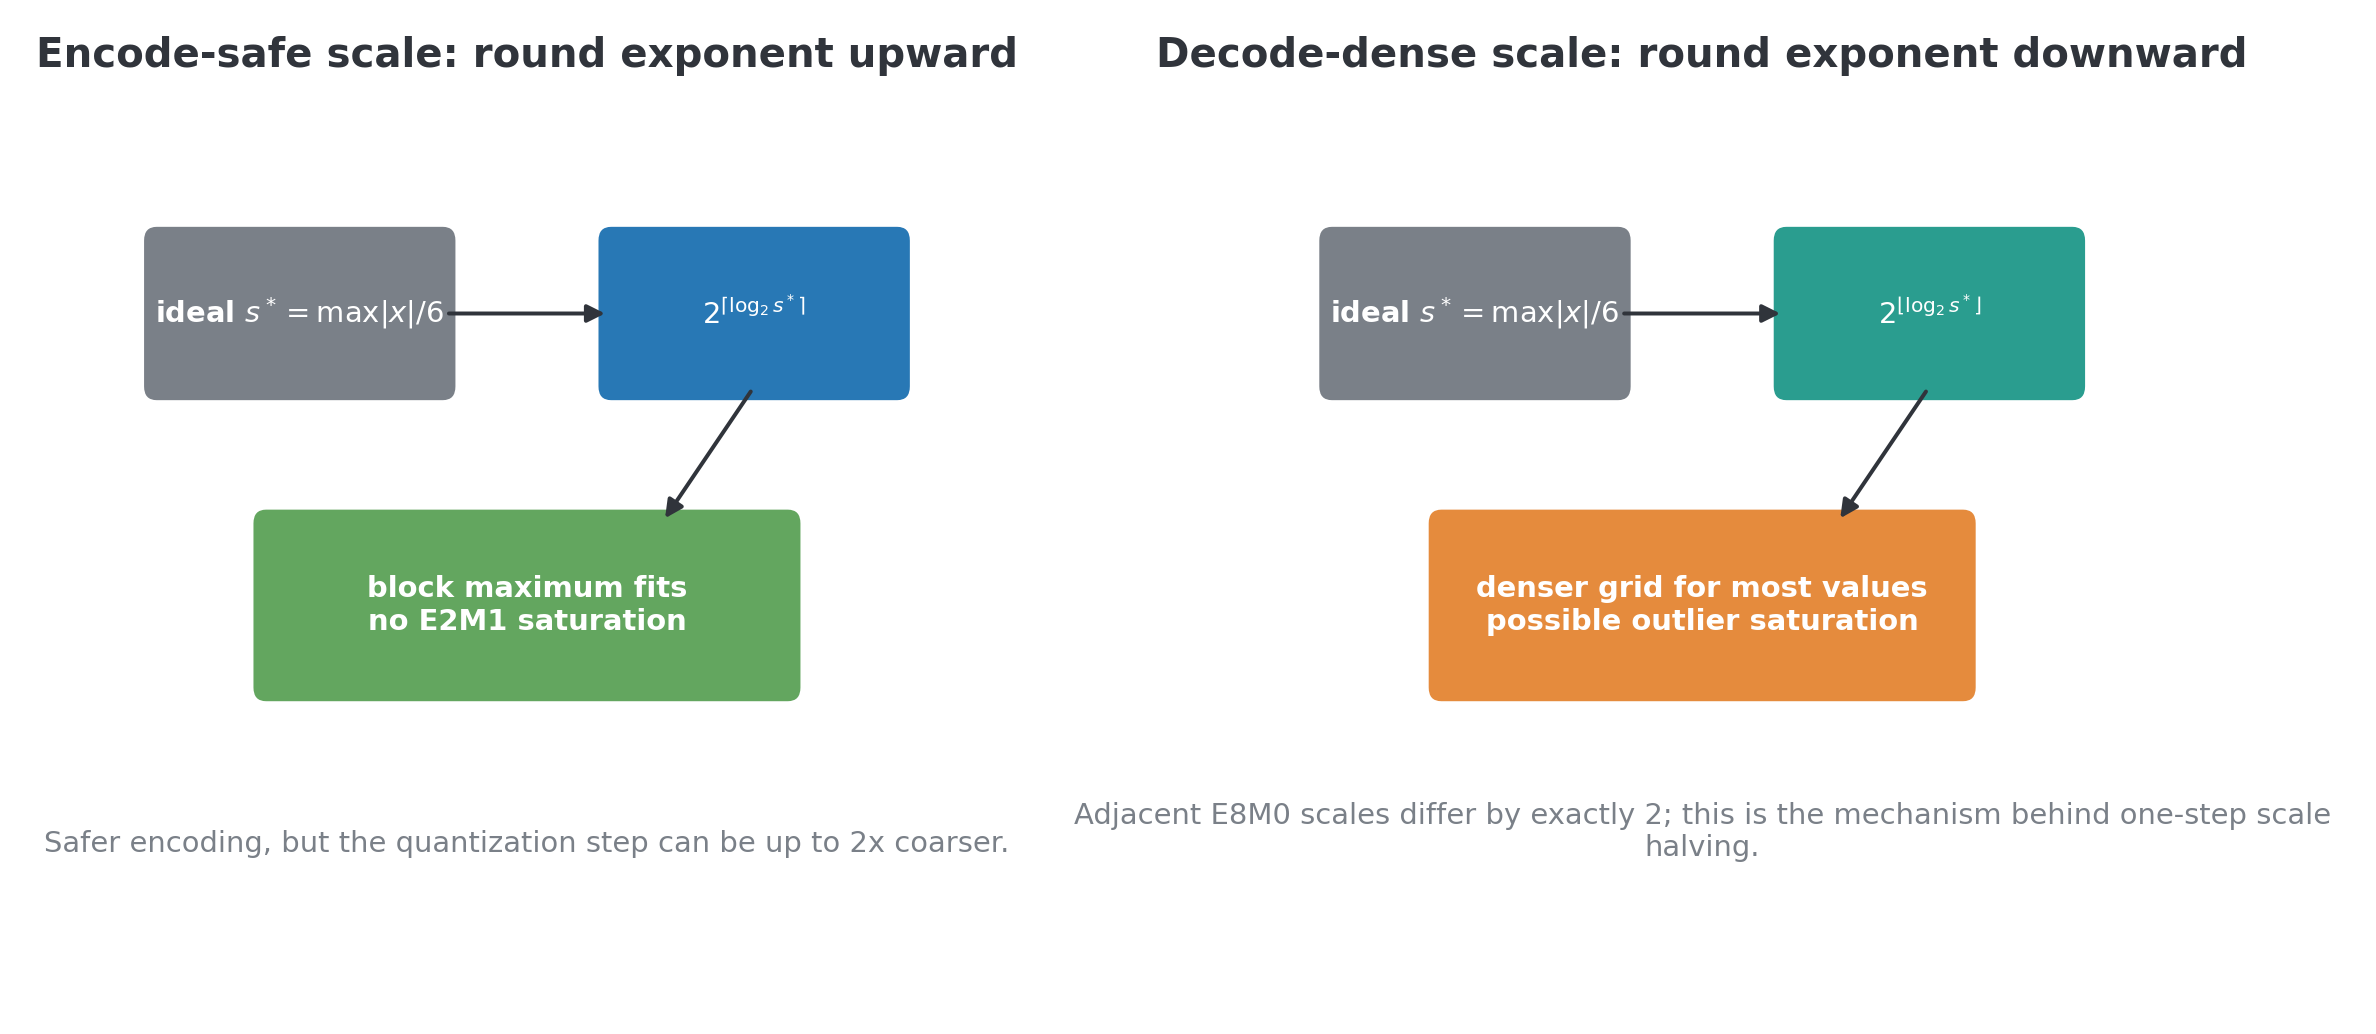
\includegraphics[width=0.96\textwidth]{figures/fp4_mxfp4_scale_rounding.png}
  \caption{Encode- and decode-centric E8M0 scale selection. Encode-centric
  scaling rounds the block maximum upward and keeps every input within the
  E2M1 endpoint. For a non-power-of-two maximum, decode-centric scaling rounds
  downward, halves the decoded grid spacing, and clips the block tail. The
  reported activation and gradient paths use the encode-centric rule. The
  2D32 weight path selects the smaller scale only under the fixed
  $a_T/s_T<0.87$ condition.}
  \label{fig:mxfp4-scale-rounding}
\end{figure}

Global \nvfp{} instead uses an E4M3 scale for
each 16 values and an FP32 tensor scale $S$ \cite{ocp2023mx,nvidia2025nvfp4}.
Its local grid is finer, but every block depends on the completed tensor amax,
the maximum absolute value.
Our global-v5 path preserves that numerical contract while replacing generic
quantize--layout--GEMM boundaries with native producers and consumers. Here,
``v5'' names an implementation generation; it is not a different NVFP4
datatype.

The CTA-local route changes only the outer-scale domain. CTA denotes the
cooperative thread array that owns a tile. For one GEMM output tile, an A-row
tile owns $\alpha_i$ and a B-column tile owns $\beta_j$.
Both remain fixed over the complete K reduction.  If $\widetilde A$ and
$\widetilde B$ denote E2M1 values decoded with their E4M3 per-block scales,
often called microscales, then
\begin{equation}
  C_{ij}=\alpha_i\beta_j
  \sum_k \widetilde A_{ik}\widetilde B_{kj}.
  \label{eq:localcta}
\end{equation}
The Tensor Core accumulates the inner sum and the epilogue applies
$\alpha_i\beta_j$ once.  This factorization is valid only because the two
outer scales are invariant in $K$, the contraction dimension. Keeping both corrections in FP32 metadata
also avoids quantizing those corrections onto the coarser FP8 scale grid.

\begin{figure}[tbp]
  \centering
  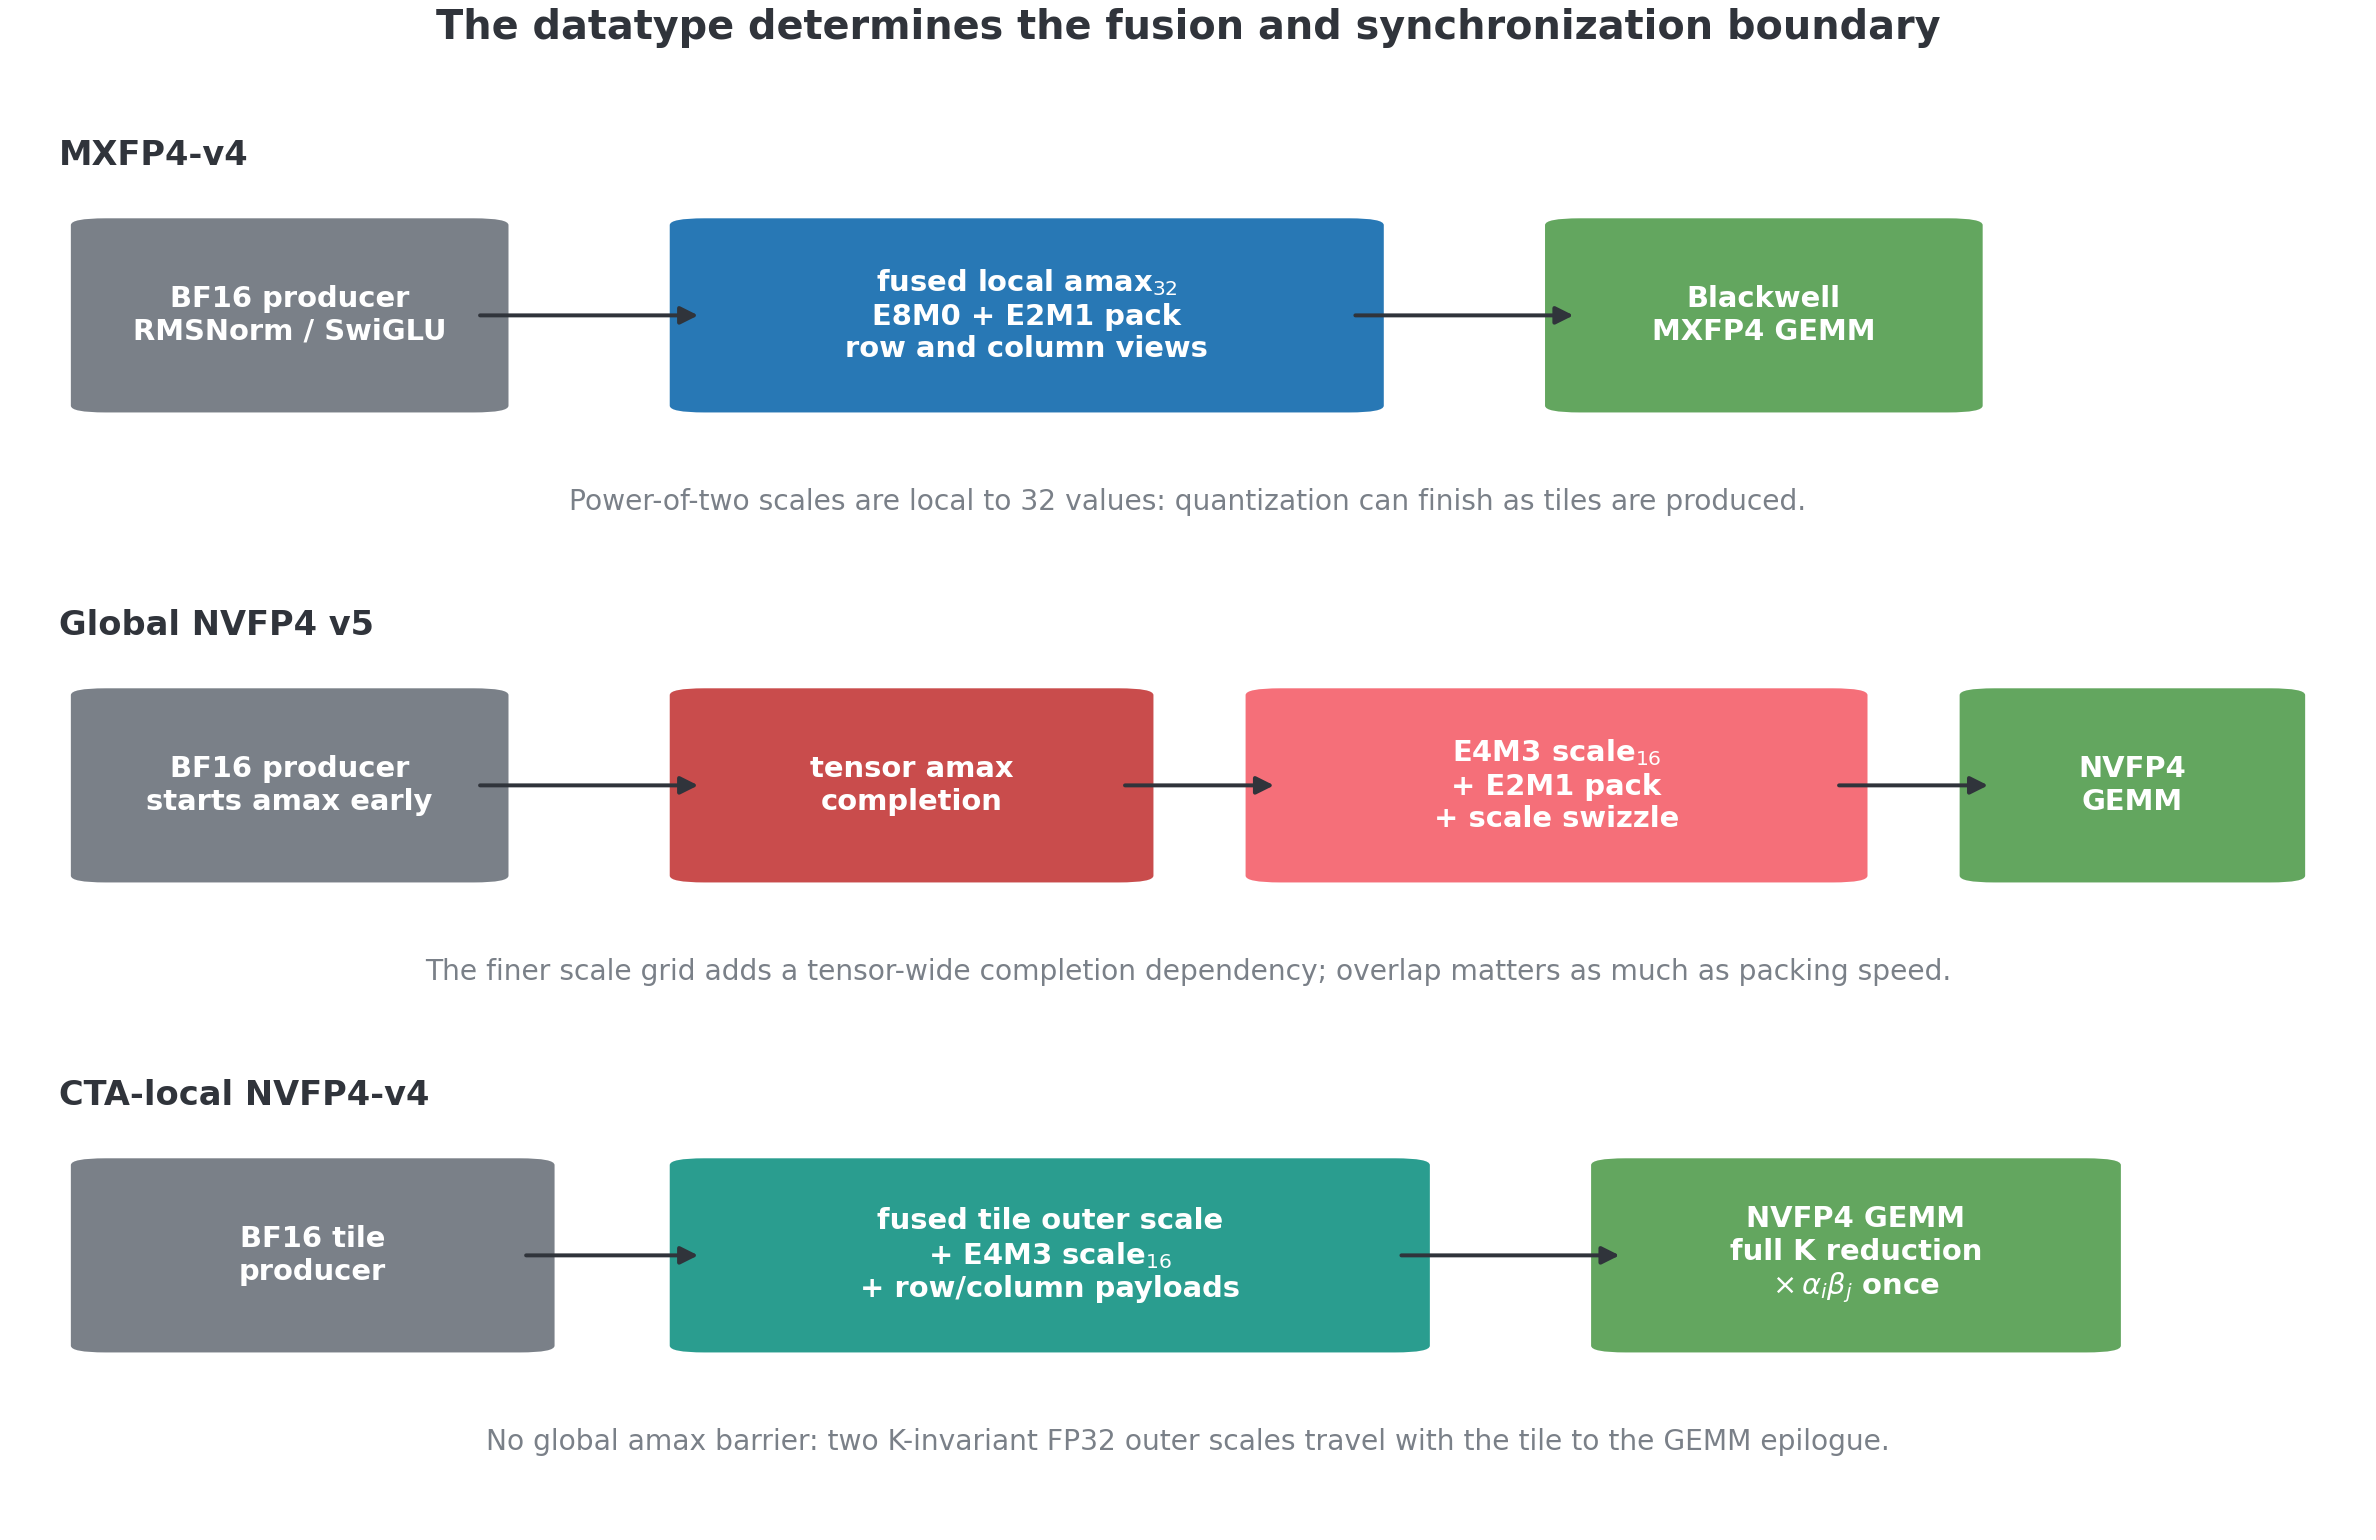
\includegraphics[width=0.98\textwidth]{figures/fp4_format_execution_routes.png}
  \caption{The formats share E2M1 payloads but expose different completion
  dependencies.  Consequently, the profitable fusion boundary is
  format-specific rather than a single generic ``FP4 linear'' kernel.}
  \label{fig:format-execution-routes}
\end{figure}

\begin{figure}[tbp]
  \centering
  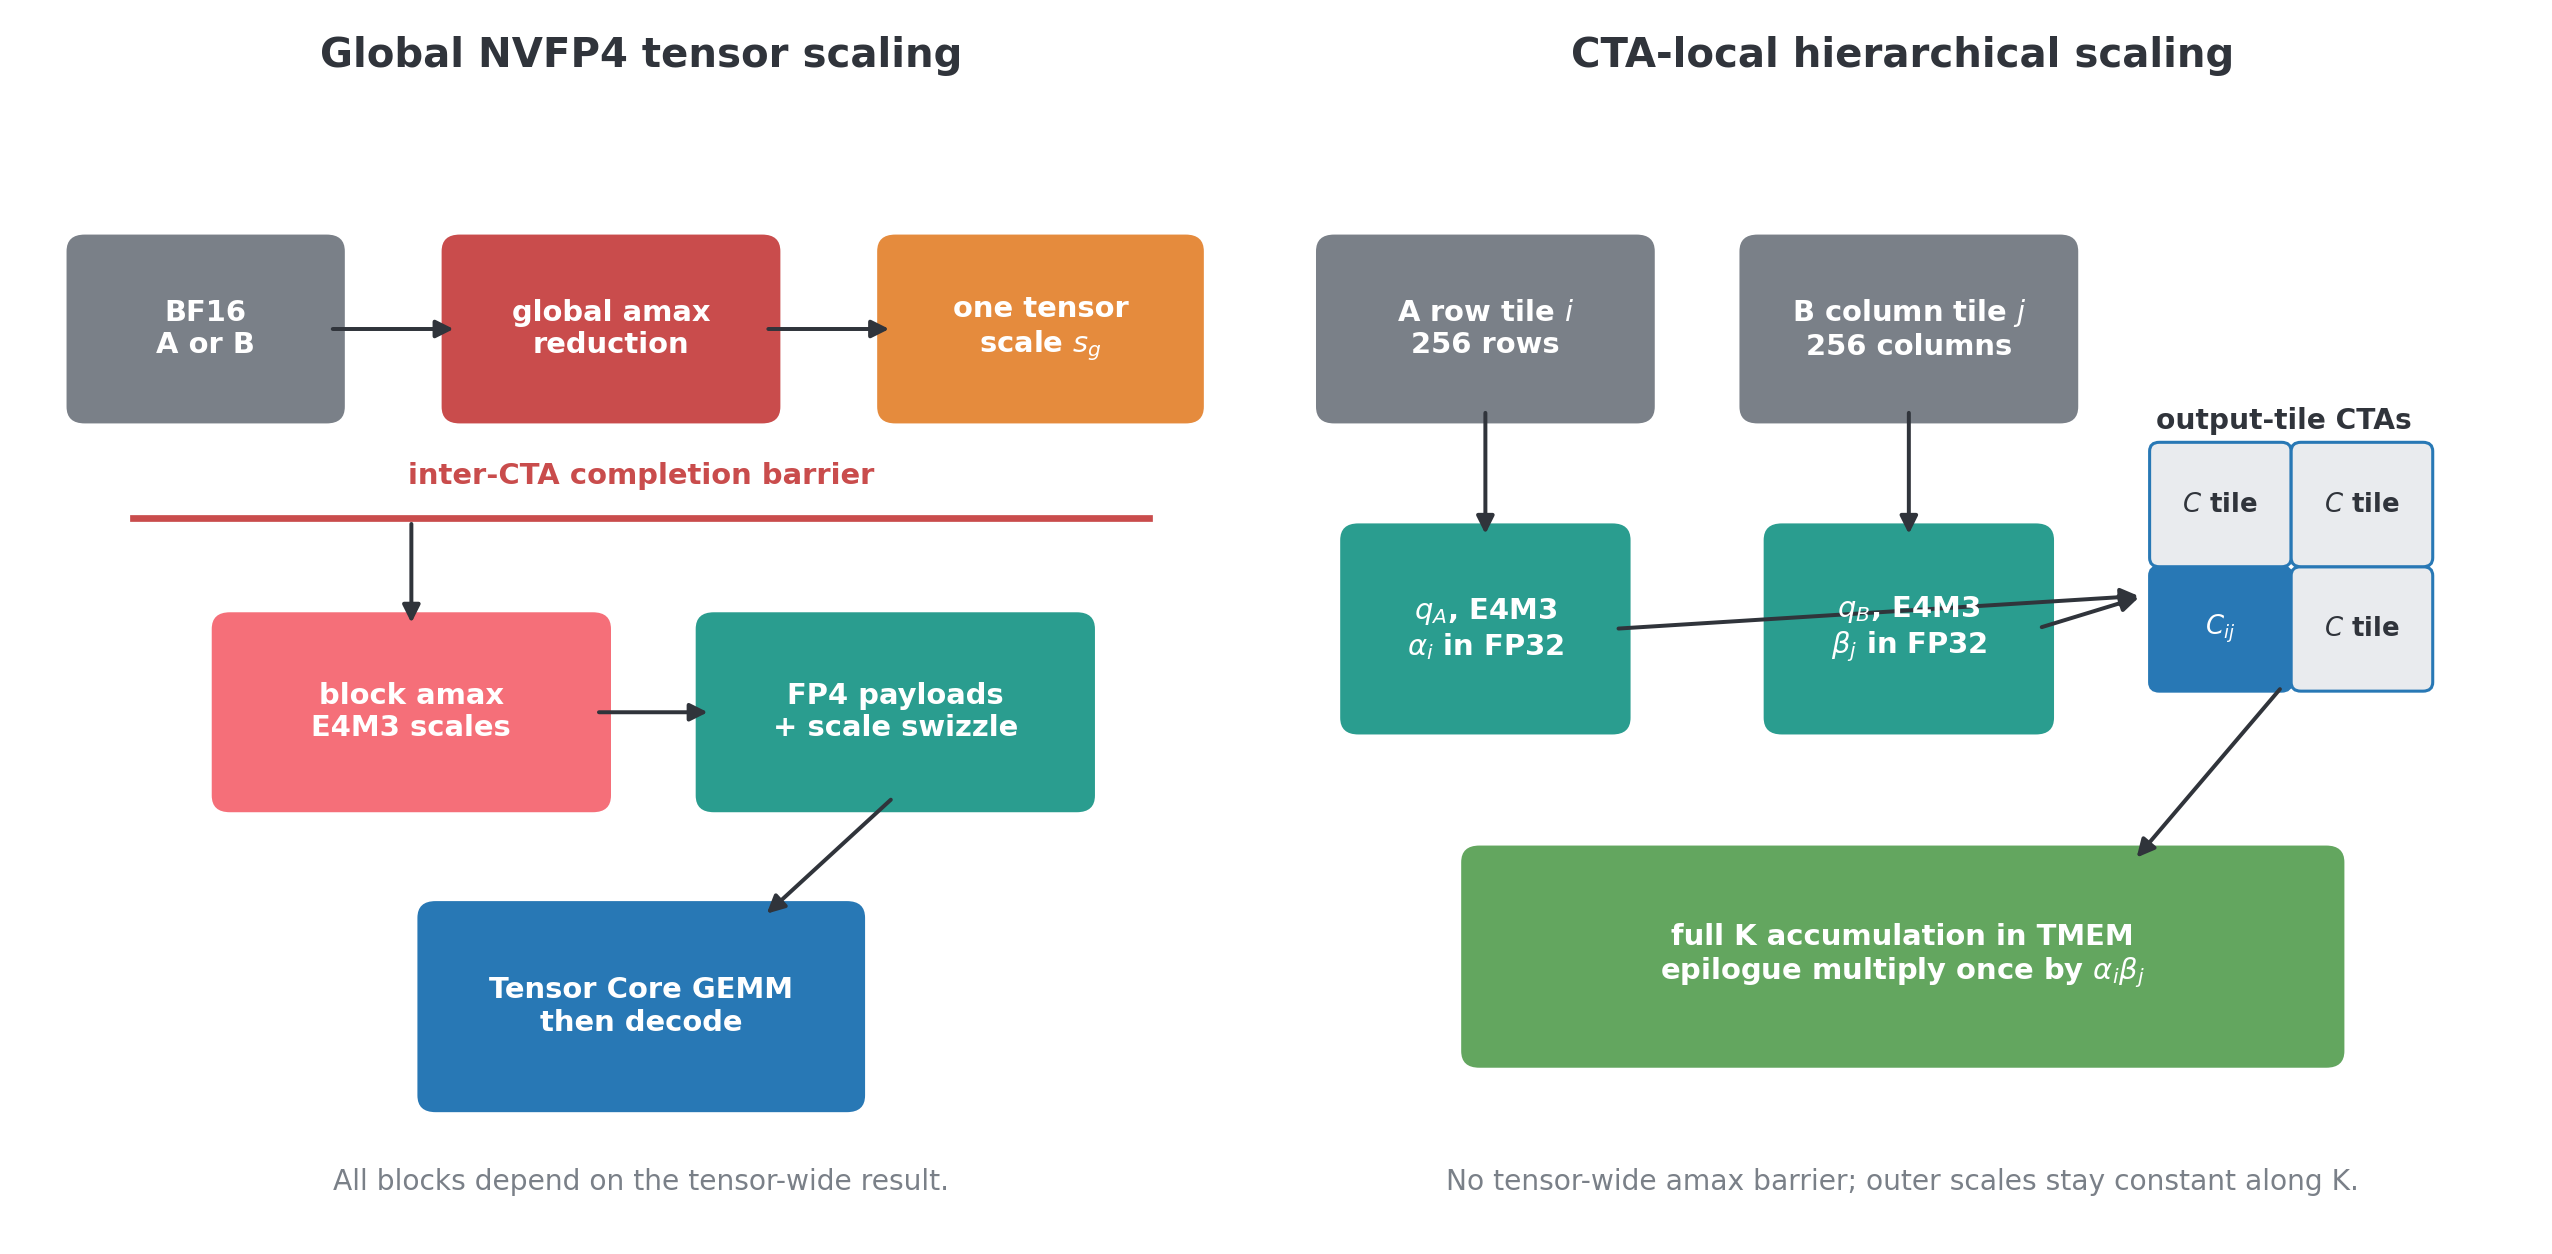
\includegraphics[width=0.94\textwidth]{figures/fp4_localcta_scaling.png}
  \caption{Global and CTA-local hierarchical \nvfp{} scaling. Global NVFP4
  completes a tensor-wide amax before finalizing its payload. CTA-local
  scaling carries row and column outer scales into the consuming GEMM and
  applies their product after the full K accumulation.}
  \label{fig:localcta-scaling}
\end{figure}

\subsection{Why forward, data gradient, and weight gradient need different views}

For a linear layer $Y=XW^{\mathsf T}$, forward propagation (Fprop), the input
or data gradient (Dgrad), and the weight gradient (Wgrad) consume different
views of the same tensors. Let $Q_r$ denote a row-facing representation and
$Q_c$ a column-facing representation. Both preserve the logical tensor shape;
the subscript identifies the physical layout and scale orientation used by the
consumer. Suppressing decode and scale metadata, training evaluates three
contractions:
\begin{align}
  \widehat Y  &= Q_r(X)Q_r(W)^{\mathsf T},
    &&\text{Fprop}, \label{eq:fprop}\\
  \widehat{dX} &= Q_r(dY)Q_c(W),
    &&\text{Dgrad}, \label{eq:dgrad}\\
  \widehat{dW} &= Q_c(dY)^{\mathsf T}Q_c(X),
    &&\text{Wgrad}. \label{eq:wgrad}
\end{align}
Thus one saved gradient needs a row-oriented payload for Dgrad and a
column-oriented payload for Wgrad; weights likewise participate in two
orientations. ``Quantize the tensor to FP4'' is incomplete unless it also
states which contraction consumes it.

\begin{figure}[tbp]
  \centering
  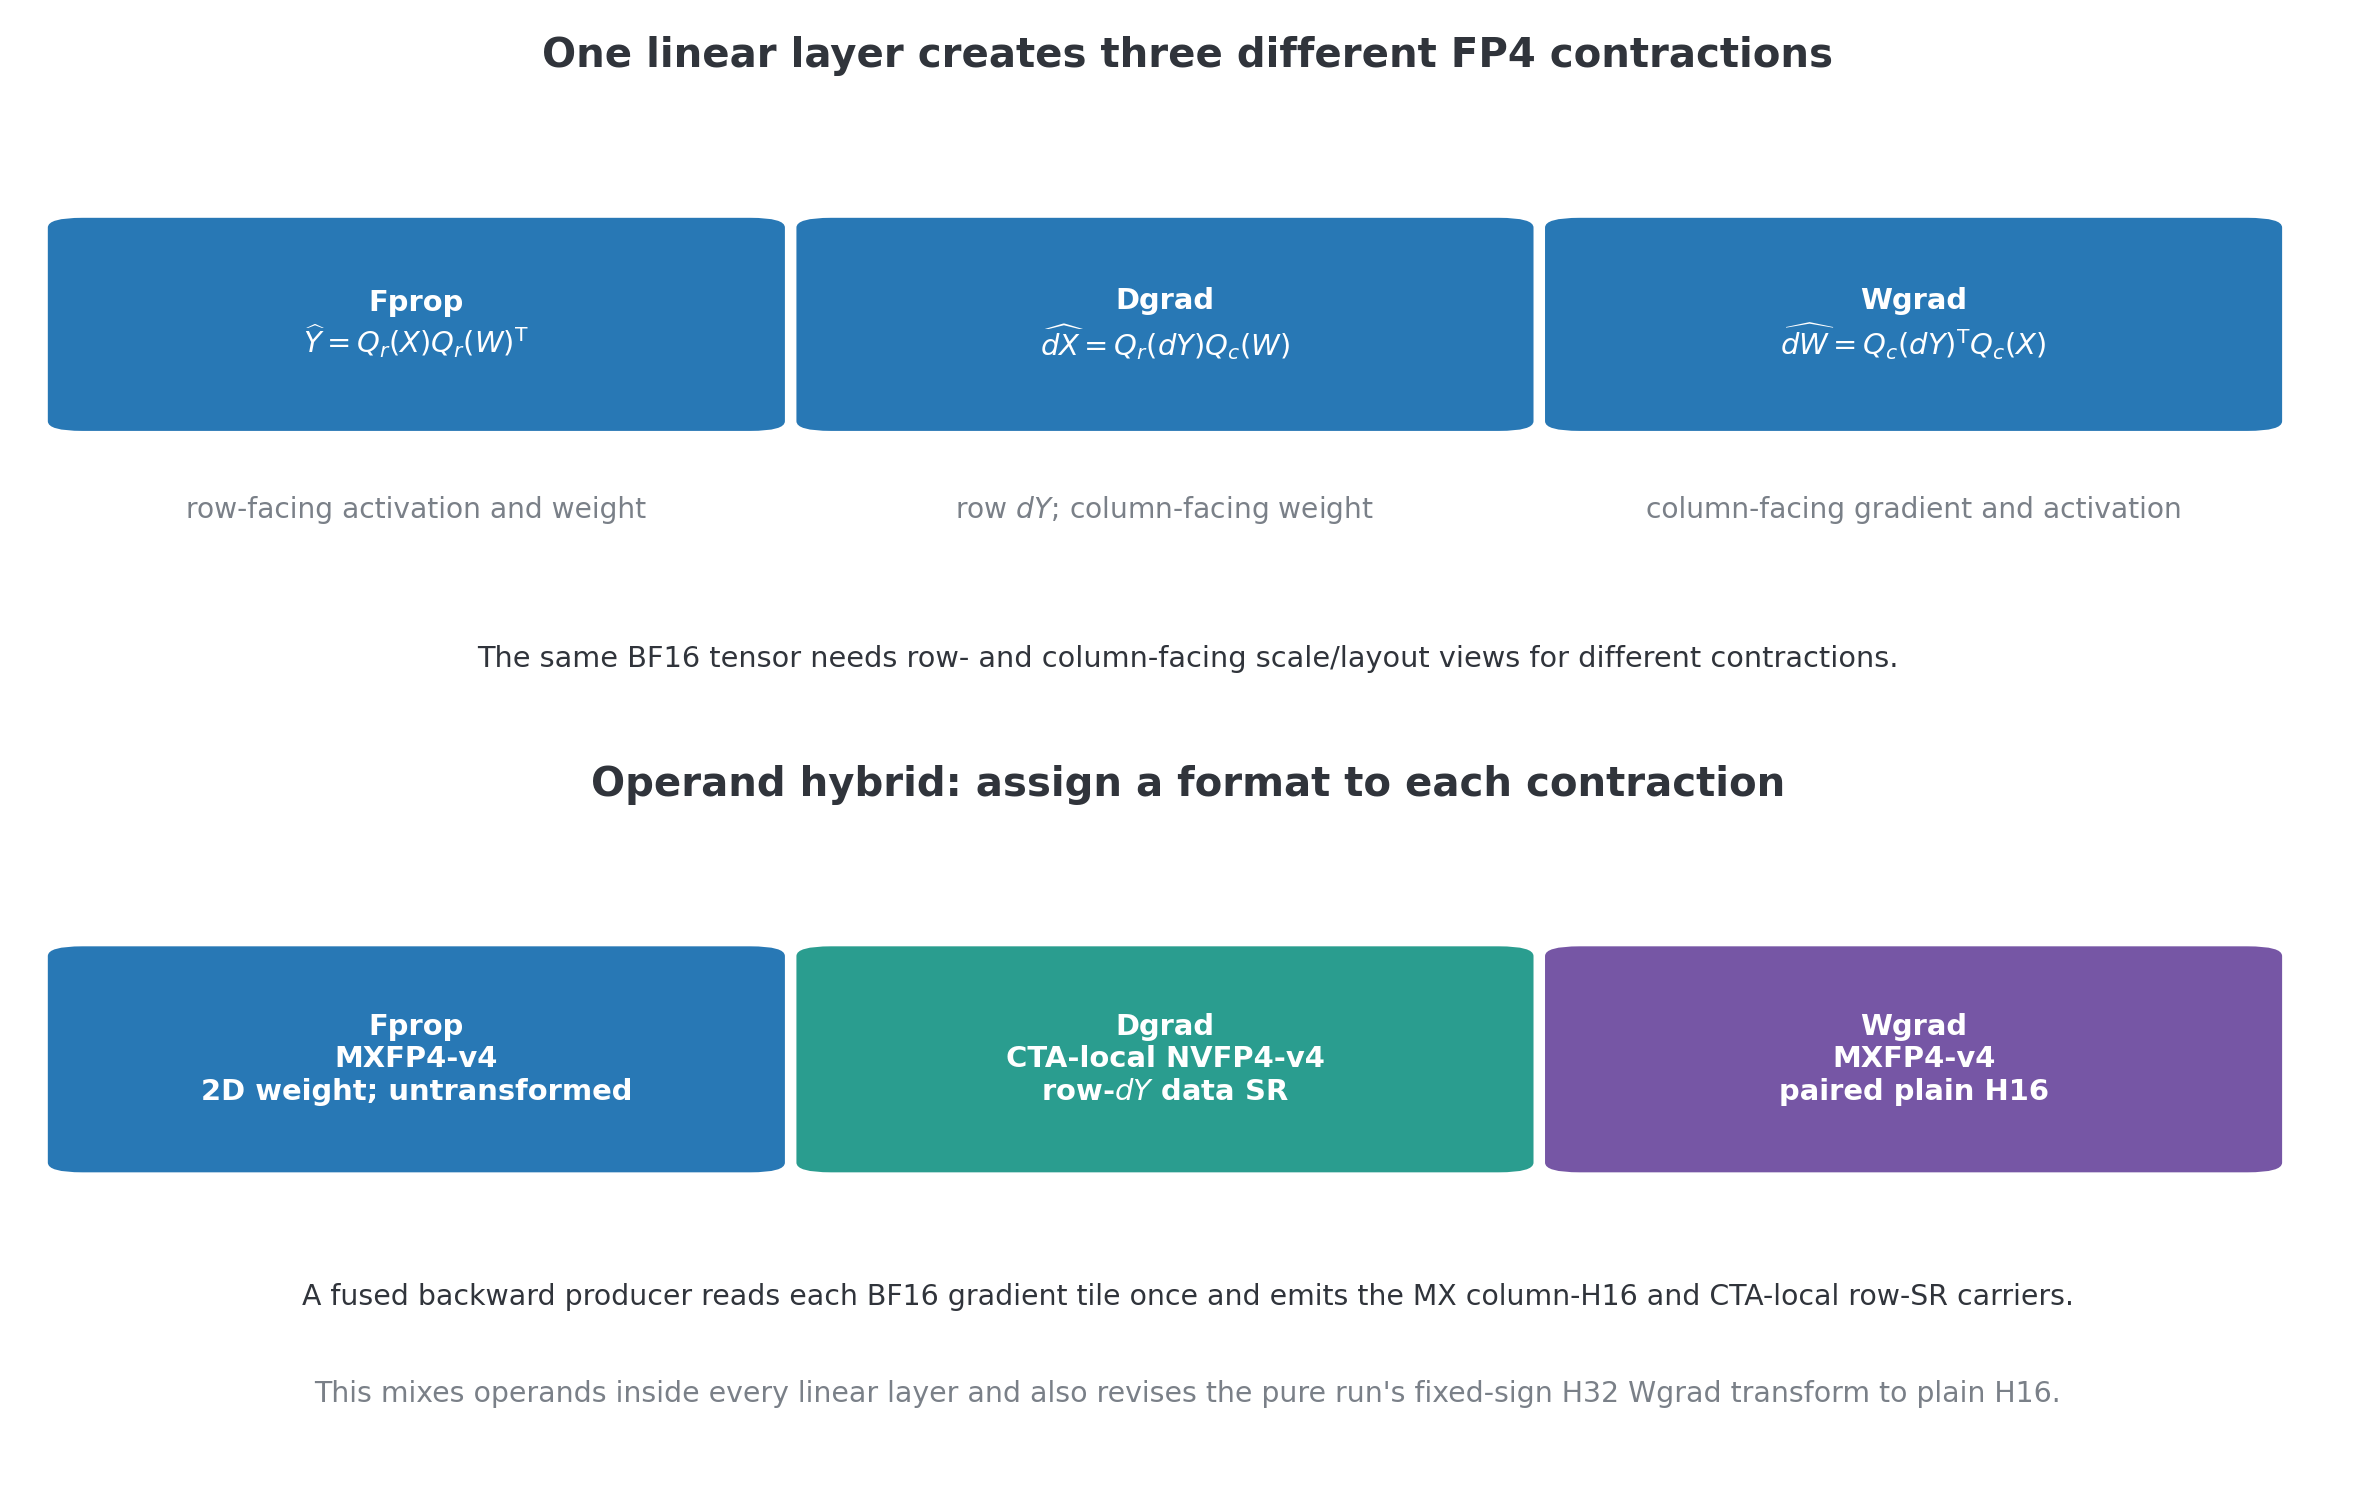
\includegraphics[width=0.97\textwidth]{figures/fp4_linear_operand_hybrid.png}
  \caption{Operand contracts for a linear layer and for the plain-H16
  operand-wise hybrid. ``Plain H16'' means a block-16 Hadamard with $D=I$ and
  no sign flips. The hybrid changes Dgrad inside every linear layer;
  it is distinct from the earlier experiment that assigned whole transformer
  blocks to different formats.}
  \label{fig:linear-operand-map}
\end{figure}

\subsection{Two-dimensional weights: numerical consistency versus implementation}

Independent one-dimensional weight quantizers can produce
$W_{\mathrm{fwd}}=Q_K(W)$ for Equation~\ref{eq:fprop} and a different
$W_{\mathrm{bwd}}=Q_N(W)$ for Equation~\ref{eq:dgrad}. Forward and backward
then consume different numerical approximations of the same BF16 weight.
Two-dimensional weight quantization instead assigns one scale to each
$b\times b$ weight tile. Let $q_{\max}$ be the largest finite E2M1 magnitude
and let $\operatorname{scale}_{\cal S}$ denote the route's scale-selection
rule on its representable scale set $\cal S$. Then
\begin{equation}
  a_{pq}=\max_{i\in p,j\in q}|W_{ij}|, \qquad
  s_{pq}=\operatorname{scale}_{\cal S}
  \!\left(\frac{a_{pq}}{S q_{\max}}\right), \qquad
  \widehat W_{ij}=S\,s_{pq}
  Q_{\mathrm{E2M1}}\!\left(\frac{W_{ij}}{S\,s_{pq}}\right),
  \label{eq:2d-weight}
\end{equation}
and reuses that numerical encoding in both orientations. The row and column
layouts can differ in memory, but their decoded weight values agree. This is
the consistency motivation identified by NVIDIA and by work on
transposition-invariant block quantization
\cite{nvidia2025nvfp4,rahimifar2026transposition}.
Equivalently, the numerical invariant is
\begin{equation}
  Q_r^{\mathrm{2D}}(W)\equiv Q_c^{\mathrm{2D}}(W)\equiv\widetilde W,
  \label{eq:2d-weight-invariant}
\end{equation}
even though the two consumer descriptors have different byte layouts.

\begin{figure}[tbp]
  \centering
  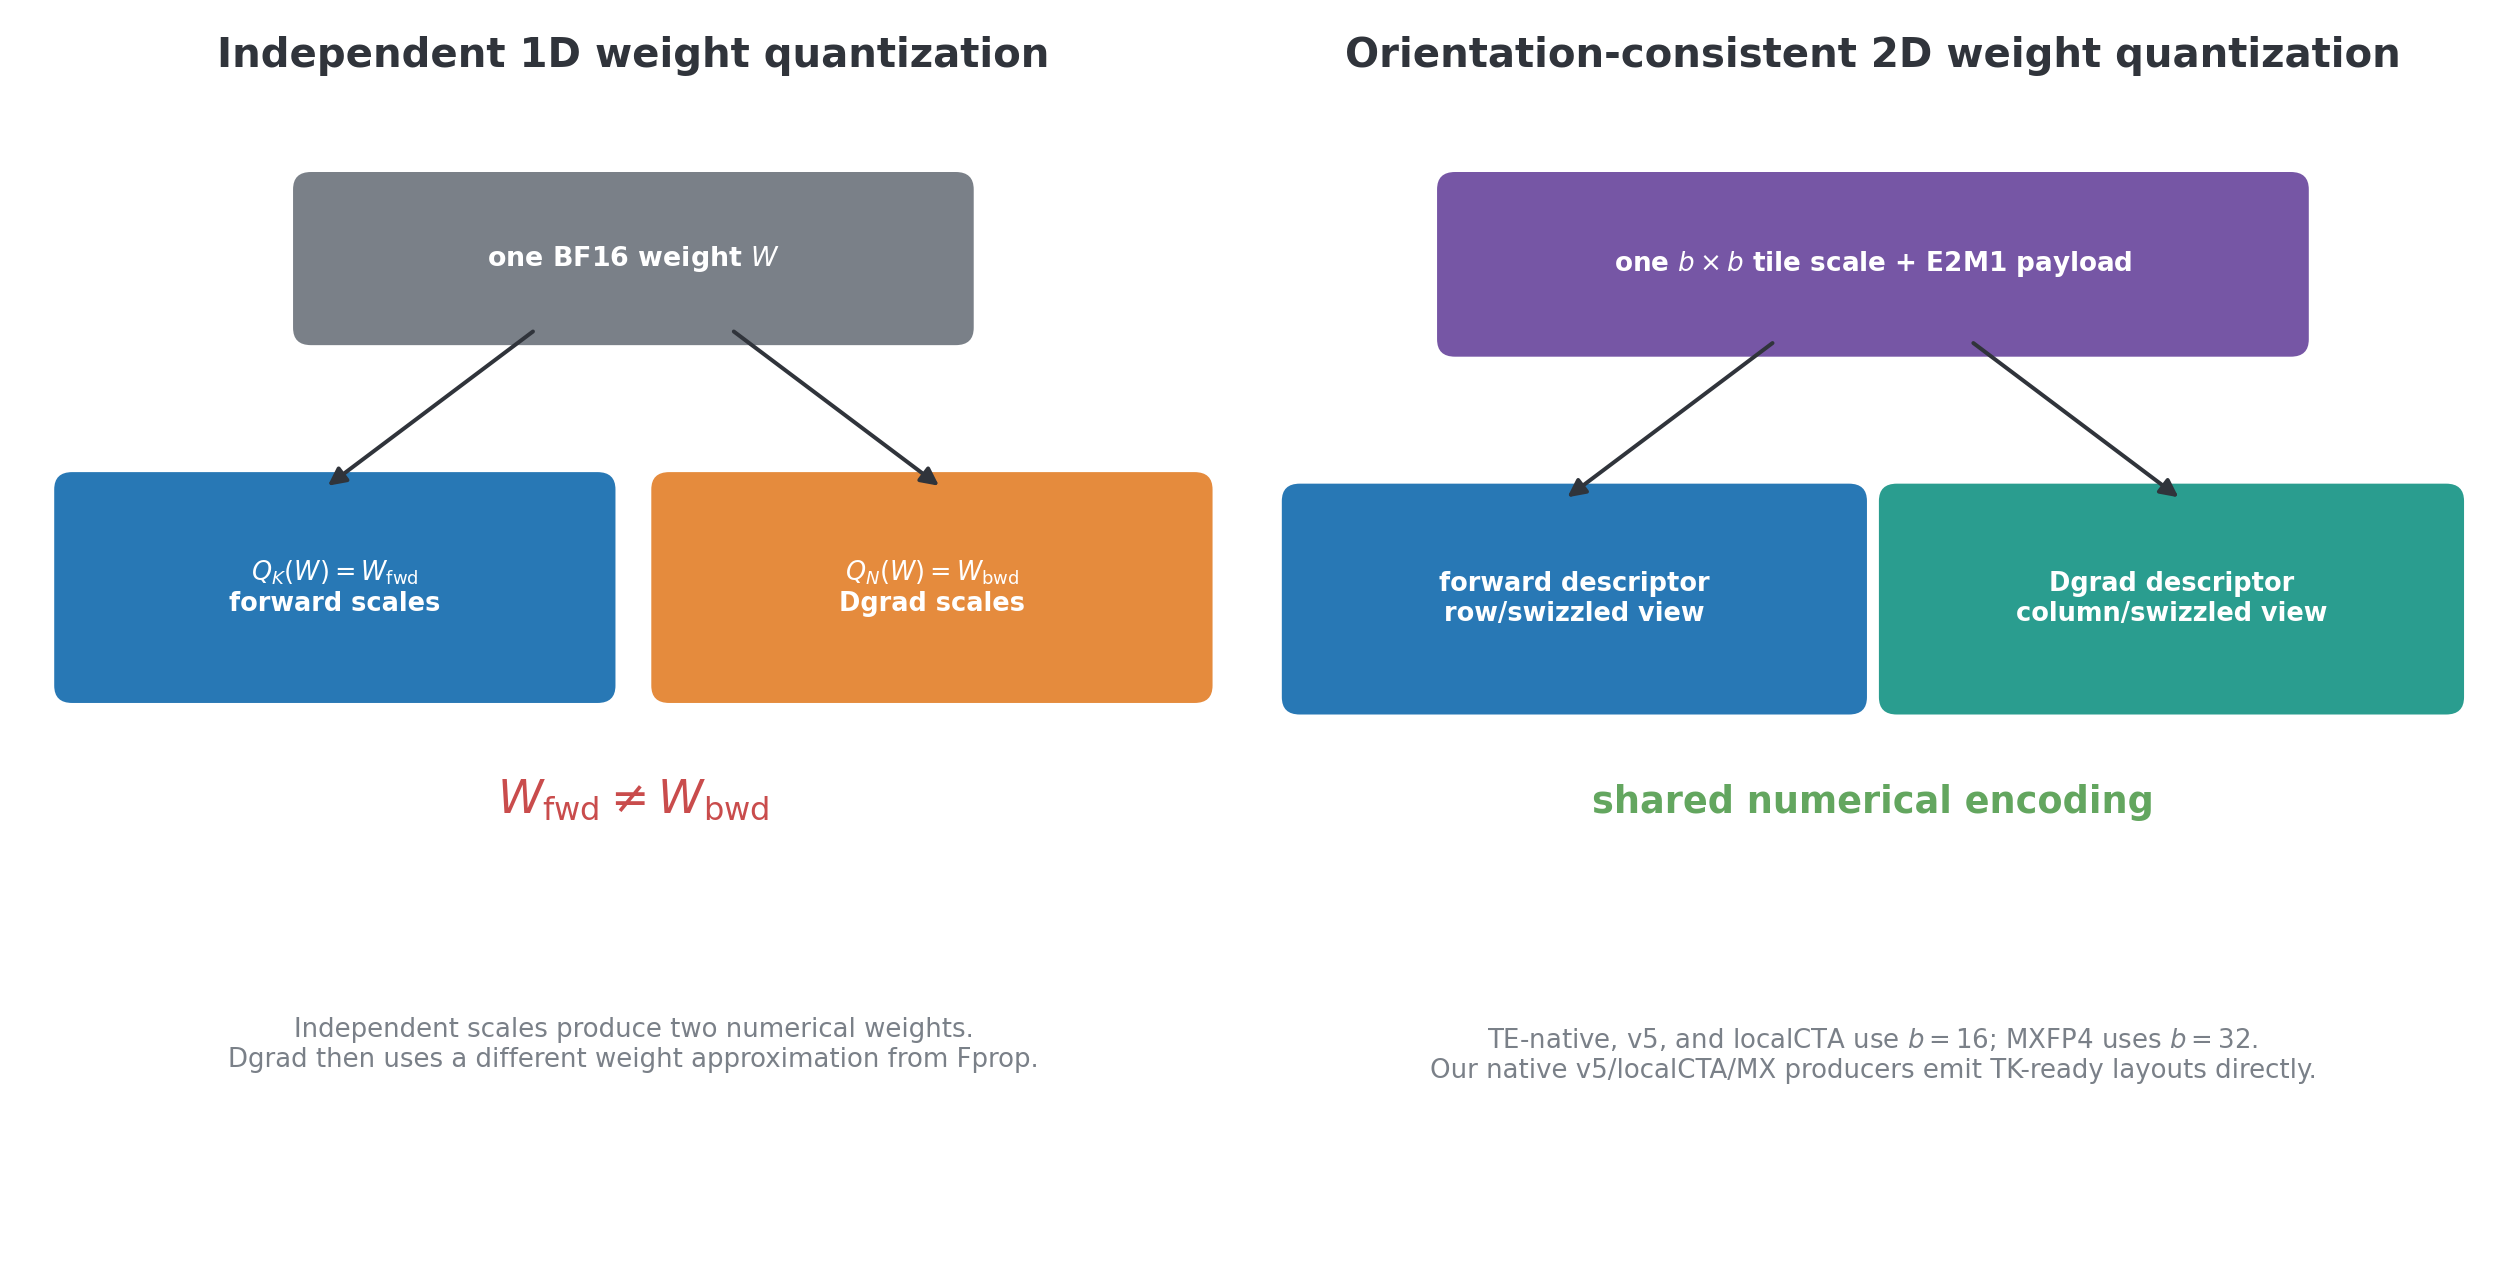
\includegraphics[width=0.96\textwidth]{figures/fp4_2d_weight_contract.png}
  \caption{One-dimensional quantization can make forward and backward see
  different weights.  A 2D tile owns one numerical encoding and exposes two
  consumer layouts.}
  \label{fig:2d-weight-contract}
\end{figure}

Transformer Engine (TE), global v5, and the CTA-local path all preserve one
numerical weight encoding across the two $16\times16$ consumer orientations.
In TE's 2D16 contract, one scale belongs to each $16\times16$ weight tile and
is replicated into the $1\times16$ scale descriptors required by the Tensor
Core consumers \cite{nvidia2025nvfp4,nvidia2026te}. ``2D'' therefore describes
shared numerical scale ownership, not a new matrix-multiplication shape. TE and
global v5 use the tensor-level NVFP4 outer scale; global v5 emits the
E2M1 values, scale metadata, and consumer layouts directly instead of
materializing TE descriptors. CTA-local NVFP4 keeps the 2D16 consistency
invariant but replaces the tensor outer scale with the tile-owned factors in
Equation~\ref{eq:localcta}. Our \mxfp{} path applies the same
orientation-consistency objective to $32\times32$ MX tiles. Tseng et al.'s
backward-only MXFP4 method instead
quantizes each operand along the reduction axis of the current contraction
\cite{tseng2025mxfp4}. Transpose-consistent 2D32 MXFP4 is prior art
\cite{cim2026nativemxfp4}; our contribution is to generate both consumer
layouts inside the fused Llama execution path.

Equation~\ref{eq:2d-weight-invariant} applies to the pure routes and the
depth-wise hybrid. The operand-wise hybrid is an explicit exception: it reads
the BF16 weight once, then emits a 2D32 MX weight encoding for Fprop and a 2D16
CTA-local weight encoding for Dgrad. Wgrad does not consume $W$; it separately
quantizes $X$ and $dY$ with MXFP4. This gives each contraction a different
error profile, so end-to-end training must evaluate the tradeoff.

\subsection{Stochastic rounding and signed Hadamard preconditioning}

For adjacent representable values $q_-$ and $q_+$, data stochastic rounding
(SR) uses
\begin{equation}
  \Pr[Q_{\mathrm{SR}}(z)=q_+]
  =\frac{z-q_-}{q_+-q_-}, \qquad
  \Pr[Q_{\mathrm{SR}}(z)=q_-]=1-\Pr[Q_{\mathrm{SR}}(z)=q_+],
  \label{eq:sr}
\end{equation}
which is unbiased between the two grid points before saturation
\cite{gupta2015limited,ozkara2025sr}. This is the ideal probability rule;
implementations that use too few random bits can introduce bias
\cite{fitzgibbon2025fewbits}. Equation~\ref{eq:sr} is ordinary adjacent-bin SR,
not LUQ. LUQ also stochastically handles values below the logarithmic FP
minimum and selects the range to avoid clipping \cite{chmiel2023accurate}. Our
microscaled E2M1 paths can saturate, so we claim removal of deterministic bias
between adjacent finite values, not unbiasedness of the complete saturated
quantizer.

The placement also differs. FP4 All the Way applies SR to the neural gradient
entering Dgrad and to both the neural-gradient and activation operands entering
Wgrad \cite{chmiel2025fp4alltheway}. NVIDIA recommends round-to-nearest for
weights and activations and SR for the gradient input to both Dgrad and Wgrad
\cite{nvidia2025nvfp4}. Our custom long routes are narrower: data SR is enabled
only on the row-oriented $dY$ representation consumed by Dgrad. The Wgrad
column representation of $dY$, weights, activations, and all scale values
remain deterministic. This axis-selective placement is a route choice evaluated
here, not a new stochastic estimator.

Hadamard preconditioning addresses a different failure mode. One outlier can
set the scale for a whole block, leaving fewer useful E2M1 values for the other
entries. A Hadamard transform mixes the block with additions and subtractions
before quantization, spreading a large coordinate over the block. In Wgrad,
this can keep smaller contributions from underflowing to zero. The transform
must be applied to both inputs of the weight-gradient dot product so that it
cancels in exact arithmetic
\cite{ashkboos2024quarot,tseng2025mxfp4,nvidia2025nvfp4}. If $H$ is the
normalized block Hadamard matrix and $R=HD$ uses a sign diagonal $D$, then
\begin{equation}
  dW=dY^{\mathsf T}X=(R dY)^{\mathsf T}(R X),
  \qquad R^{\mathsf T}R=I.
  \label{eq:paired-rht}
\end{equation}
Both Wgrad operands must therefore be transformed as a pair. Transforming only
$dY$ changes the gradient rather than only changing its quantization basis.

The Hadamard matrix itself is deterministic. In a randomized Hadamard
transform (RHT), ``randomized'' refers to how the signs in $D$ are selected;
it does not require a new sign draw at every optimizer step. Tseng et al.
sample signs and transform both MXFP4 backward GEMMs:
$(dY,W)$ for Dgrad and $(dY,X)$ for Wgrad, using a 64-value transform in their
main experiments \cite{tseng2025mxfp4}. NVIDIA's NVFP4 recipe instead
transforms Wgrad only, using a 16-value Hadamard (H16) for NVFP4 and a 32-value
Hadamard (H32) for its MXFP4 comparison
\cite{nvidia2025nvfp4,nvidia2026te}. NVIDIA samples one sign vector and shares
it across linear layers and training steps; it is fixed during the run but
random at setup \cite{nvidia2025nvfp4}. H16 and H32 name the number of values
mixed by the transform.

Our custom kernels instead specify one sign diagonal as part of the route. H16
uses a fixed 16-entry pattern, and H32 repeats that motif over two 16-value
halves. No sign vector is sampled at setup or during training. We therefore
call these paths \emph{fixed-sign H16/H32
preconditioning}, rather than RHT. The additions and subtractions mix
the values; the fixed signs choose which values are negated first. Applying
the same transform to $X$ and $dY$ preserves the unquantized Wgrad dot product,
and the stored weight is never transformed. A fixed $D$ remains orthogonal and
repeatable across layers, steps, and resumes. It does not, however, inherit a
probabilistic concentration guarantee that assumes $D$ is sampled independently
of its input. We neither claim that guarantee nor compare alternative sign
vectors.

Our recipe combines row-oriented SR only for Dgrad with paired fixed-sign
Hadamard preconditioning only for Wgrad. H16 matches the 16-value NVFP4 scale
block, while H32 matches the 32-value MXFP4 scale block. Deterministic Hadamard
preconditioning and transpose-consistent 2D32 MXFP4 have prior art
\cite{cim2026nativemxfp4}; the contributions here are their integration with
axis-selective SR, CTA-local two-sided scaling, and fused producer paths. The
literal sign pattern and its half-block construction are recorded in
Appendix~\ref{app:implementation}. Table~\ref{tab:recipe-state-ledger} states
the sign and rounding policy for every route.

\subsection{Reference NVFP4 recipe versus the routes evaluated here}

The NVIDIA recipe is a bundle, not only the NVFP4 datatype. It recommends
2D16 weights, SR on gradient inputs to Dgrad and Wgrad, a paired H16 signed
Hadamard transform (described as RHT) for
Wgrad, and retaining roughly 15\% of empirically sensitive linears in higher
precision, with most selected linears near the end of the network
\cite{nvidia2025nvfp4}. Three distinctions matter in this report. First, our
TE-native comparator enables TE's 2D, gradient-SR, and signed-Hadamard
mechanisms but places all 32 body blocks in NVFP4; only the common output head
is BF16. Second, the TE comparator with four final BF16 blocks is a separate
NVIDIA-inspired route. It is not a reproduction of NVIDIA's per-linear
sensitivity list. Third, the custom v5, \mxfp{}, and \localcta{} long routes
use row-Dgrad SR, and only explicitly named routes apply Hadamard
preconditioning. Tables~\ref{tab:recipe-ledger}
and~\ref{tab:recipe-state-ledger} state the complete contract for each result.
\FloatBarrier

\section{Fused Execution}
\label{sec:method}

\subsection{Fuse the complete producer--consumer boundary}

Quantization helps only when its preparation work fits under the matrix
multiplication. We model the latency of one FP4 boundary by its critical path:
\begin{equation}
  T_{\mathrm{boundary}} \approx T_{\mathrm{serial}} +
  \max\!\left(T_{\mathrm{GEMM}},
  T_{\mathrm{reduce}}+T_{\mathrm{quant}}+T_{\mathrm{layout}}\right),
  \label{eq:boundary-cost}
\end{equation}
Here $T_{\mathrm{serial}}$ is work that cannot overlap because of a data
dependency or resource contention. Fusion removes an HBM round trip only when
the producer emits every scale, layout, and saved value required by the next
operation. Accelerating only the GEMM epilogue can leave a global reduction, a
second tensor orientation, or backward recomputation on the critical path.

\begin{figure}[tbp]
  \centering
  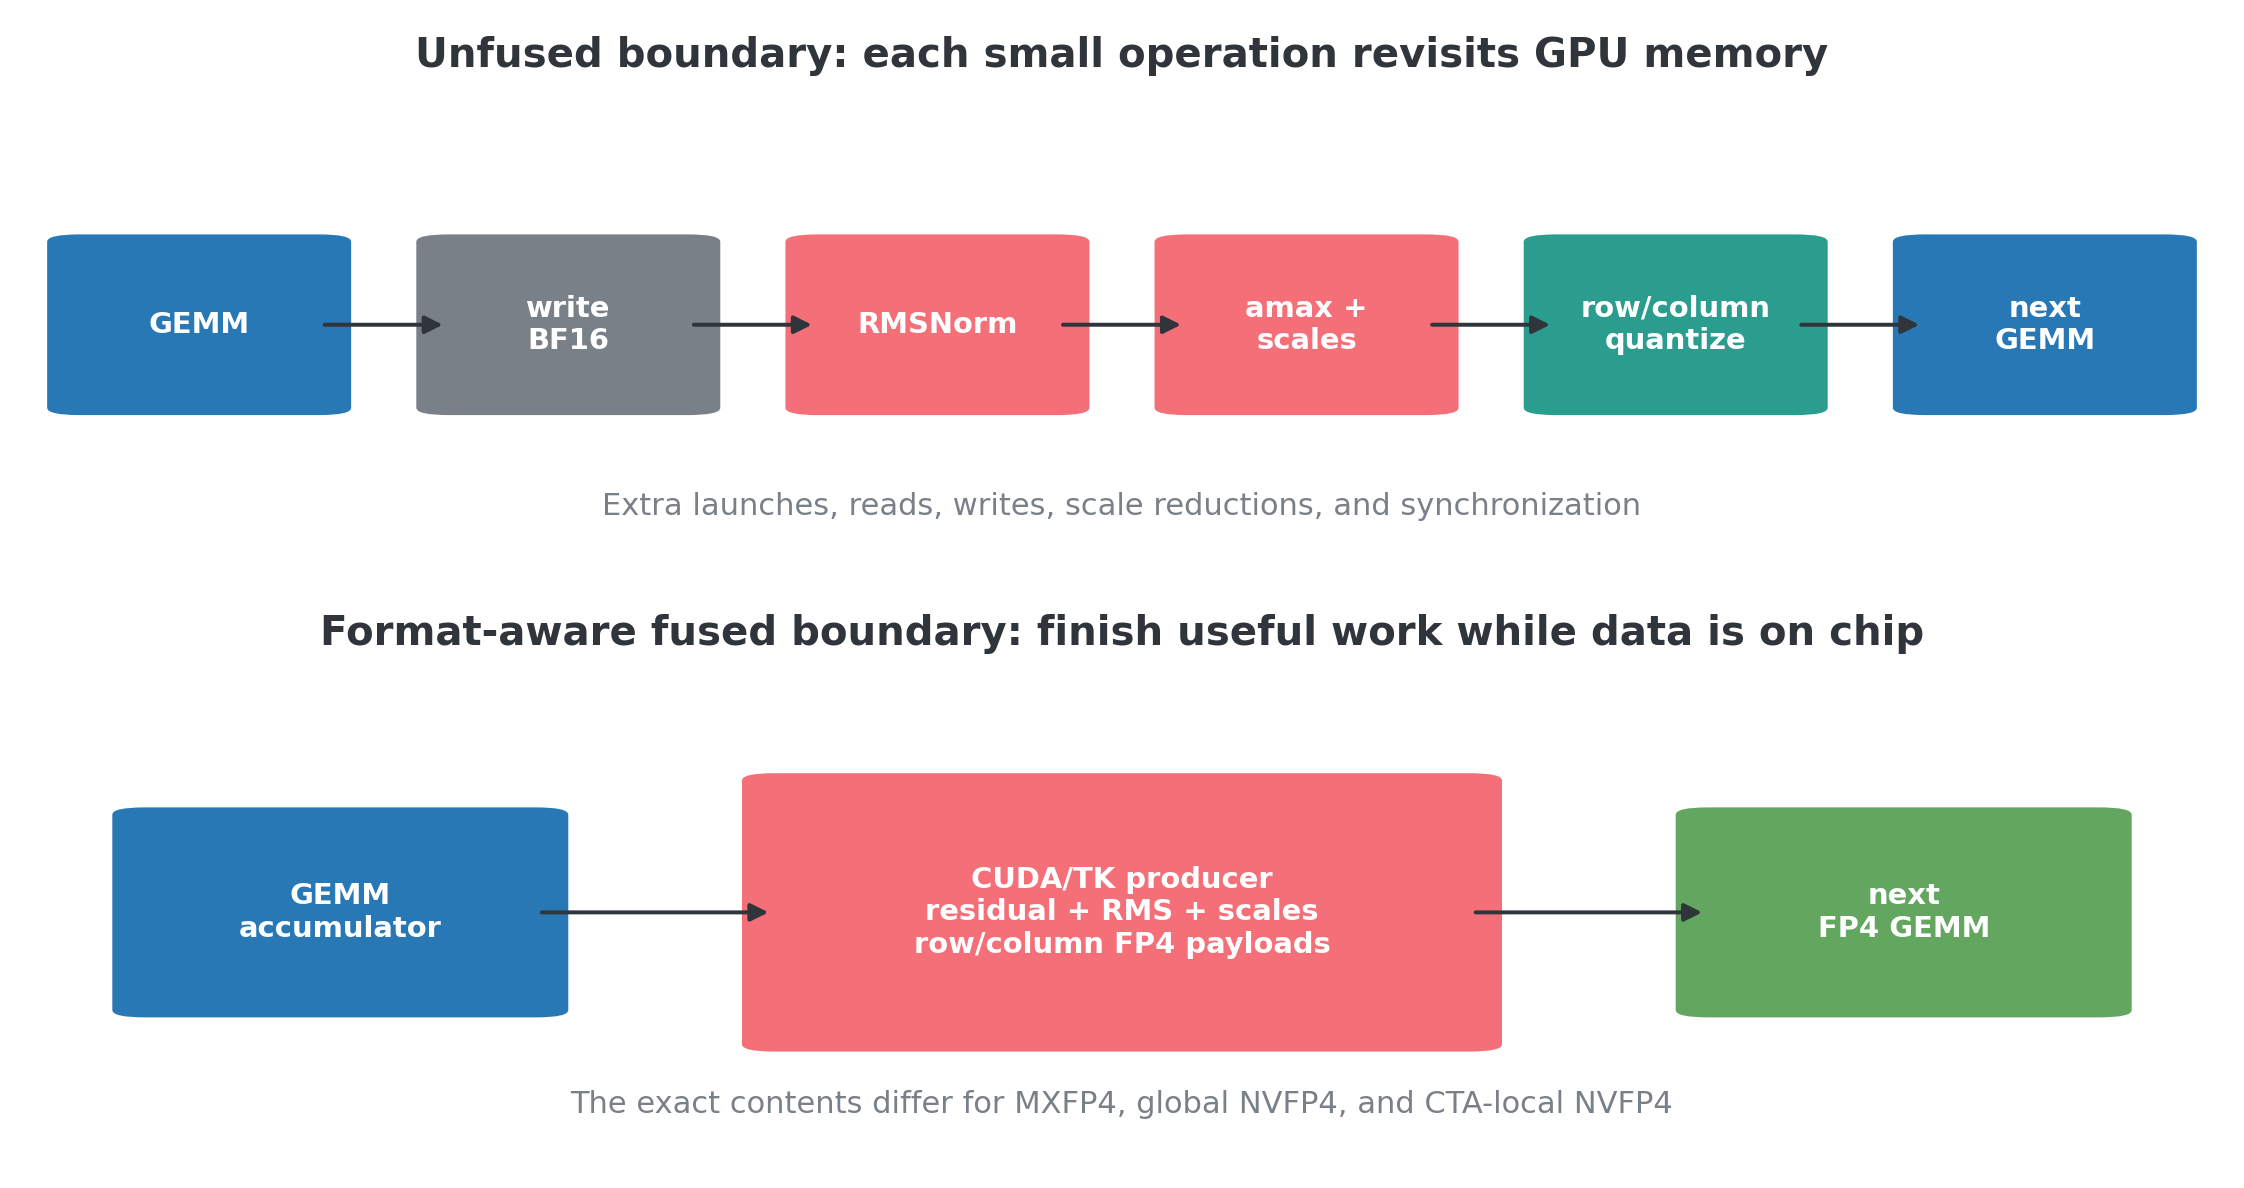
\includegraphics[width=0.93\textwidth]{figures/fp4_fusion_dataflow.png}
  \caption{Format-aware fusion treats normalization, scale production,
  physical layout, the consuming GEMM, and backward state as one execution
  boundary.}
  \label{fig:fusion-dataflow}
\end{figure}

We implement the fused tensor operations in CUDA and \tk{}
\cite{spector2024thunderkittens}. Following CODA's GEMM-plus-epilogue framing
\cite{guo2026coda}, an operation joins a boundary only when the next stage can
consume its output directly. A Llama block exposes four such boundaries:
root-mean-square normalization (RMSNorm) into the query/key/value (QKV)
projection, QKV into attention, the gated feed-forward network (FFN), and the
residual update into the next RMSNorm. Each has a corresponding backward
boundary.

\subsection{What is fused in a Llama block}

The system specializes four repeated Llama boundaries.  Table~\ref{tab:fusion-ledger}
states both the shared algebra and the format-dependent schedule.

\begin{table}[tbp]
  \centering
  \caption{High-level fusion ledger. ``Both views'' means the row and column
  representations required by Equations~\ref{eq:dgrad}
  and~\ref{eq:wgrad}.}
  \label{tab:fusion-ledger}
  \begin{tabularx}{\textwidth}{lYYY}
    \toprule
    Boundary & \mxfp{}-v4 & Global \nvfp{} v5 & \localcta{}-v4 \\
    \midrule
    RMSNorm $\rightarrow$ QKV
      & Row statistics, normalized value, local scales, and both views share a producer
      & Tensor amax starts with normalization; scale completion and layout are overlapped
      & Row/column tile outer scales and both views are emitted without a global barrier \\
    QKV $\rightarrow$ attention
      & Grouped Q/K/V GEMM; Q/K rotary position embedding (RoPE) is owned by the projection boundary
      & Same algebra with native NVFP4 payload/scale descriptors
      & Same algebra; GEMM epilogue applies the two outer corrections \\
    Gated FFN
      & W1/W3 scheduling plus sigmoid linear unit (SiLU)--gate output and the W2 input producer
      & Native 16-value quantization replaces generic TE-to-custom materialization
      & W2 Dgrad, SiLU derivative, and split W1/W3 backward representations are co-produced \\
    Residual $\rightarrow$ RMSNorm
      & Exact residual and row statistics are carried while next FP4 views are formed
      & Global-scale work is launched early rather than hidden in a nominal epilogue
      & K-invariant outer scales remain available through the consuming GEMM \\
    Backward layouts
      & One producer emits deterministic column payloads and row-SR payloads with checkpointed random state
      & One native producer emits 16-value hierarchical views and 2D-weight descriptors
      & One producer emits row/column E2M1, E4M3 per-block scales, and FP32 outer scales \\
    \bottomrule
  \end{tabularx}
\end{table}

The gated FFN illustrates why the boundary extends beyond a GEMM.
Writing W1 and W3 outputs to BF16, launching a separate SiLU--multiply, then
reading the result again to quantize W2's input spends bandwidth between every
large contraction. The fused path schedules the paired projections together
and emits W2's FP4 input with the SiLU--gate output. In backward, it combines
W2 Dgrad with the SiLU derivative and produces the representations consumed by
W1/W3 Dgrad and Wgrad. Exact BF16 values remain available where autograd
requires them; fusion changes data movement, not the model definition.

QKV follows the same principle. The normalized input producer emits the
format-specific representations consumed by the grouped projection, and the
Q/K projection applies RoPE and the required layout. Backward combines inverse
layout, RoPE, QKV gradient production, and the adjacent RMSNorm reduction when
their data dependencies align. Residual--RMSNorm retains the exact residual
and row statistics while producing the next quantized representations.

Scale work is scheduled by format. \mxfp{} reductions finish with each local
tile. Global \nvfp{} begins the tensor amax early so scale finalization can
overlap other work. \localcta{} removes that global dependency, but its two
outer scales must remain available through the full K reduction.
Figure~\ref{fig:format-execution-routes} summarizes these schedules.

\subsection{Depth-wise and operand-wise hybrids}

The \emph{depth-wise} hybrid assigns complete transformer blocks 1--27 to
\localcta{} and blocks 28--32 to \mxfp{}. Attention and FFN linears follow the
assigned block, so Fprop, Dgrad, and Wgrad never mix formats within one linear.
Both formats use orientation-consistent 2D weights and row-only gradient-data
SR; neither uses Hadamard preconditioning.

The \emph{operand-wise} hybrid instead chooses the format per contraction. A
same-state operator analysis found lower Dgrad error for \localcta{} than for
\mxfp{} in every measured layer and component. This motivates \mxfp{} for
Fprop and Wgrad and \localcta{} for Dgrad. The diagnostic and its scope are
reported in Section~\ref{sec:results} and
Appendix~\ref{app:dgrad-diagnostic}.

Concretely, every linear uses \mxfp{}-v4 for Fprop and Wgrad and
\localcta{}-v4 with row-data SR for Dgrad. One producer loads each BF16
gradient tile once and emits both the CTA-local row representation and the MX
column representation. The weight producer likewise loads BF16 $W$ once and
emits the MX forward view and the CTA-local Dgrad view.

We evaluate two Wgrad variants. The plain-H16 variant applies the same
16-value Hadamard mixing to $X$ and $dY$ with $D=I$, so it performs no sign
flips. The fixed-H32 variant applies the paired 32-value signed transform used
by the completed \mxfp{}+row-SR+fixed-H32 route. Neither variant transforms the
stored weight. Fprop, CTA-local Dgrad, weight encodings, row SR, output
projection, and loss retain the same numerical contract. Table~\ref{tab:gb200-throughput}
reports the two complete configurations; Appendix~\ref{app:implementation}
gives the exact sign mapping.

Every main custom route retains a BF16 output projection and compiled regular cross
entropy. Appendix~\ref{app:output-head} summarizes the low-precision output
heads that did not improve the end-to-end speed--numerics tradeoff.
\FloatBarrier

\section{Experimental Setup}

\subsection{Model, data, and training horizon}

The main workload is an 8B-parameter Llama-family decoder with RMSNorm,
grouped-query attention, rotary position embeddings (RoPE), and a gated
feed-forward network \cite{dubey2024llama3}. The sequence length is 8,192 and
the global batch is 512 sequences, or 4,194,304 tokens per update. A
160B-token run ends at step 38,147. Unless stated otherwise, the named
low-precision route applies to every body linear in all 32 transformer blocks.

All main custom routes use a BF16 output projection followed by
Inductor-compiled regular cross entropy. The optimizer is AdamW with a
2,000-step linear warmup to a peak learning rate of $3\times10^{-4}$; the rate
remains constant after warmup over the reported horizon. Training losses are
compared at matched optimizer steps. Each long-run recipe is represented by
one trajectory, so the comparisons do not estimate seed-to-seed variation.
Table~\ref{tab:base-training-recipe} summarizes the shared configuration; the
appendix records execution-specific details.

\begin{table}[htbp]
  \centering
  \footnotesize
  \caption{Shared Llama-8B training configuration.}
  \label{tab:base-training-recipe}
  \begin{tabularx}{\textwidth}{@{}lY@{}}
    \toprule
    Field & Effective contract \\
    \midrule
    Model & 32 blocks; width 4,096; FFN 14,336; 32 Q heads; 8 KV heads; head dimension 128; vocabulary 128,256 \\
    Position / norm & Llama-3.1 RoPE with base $500{,}000$, $8\times$ scaling, low/high frequency factors 1 and 4, and original length 8,192; RMSNorm $\epsilon=10^{-5}$ \\
    Data / tokenizer & Shuffled OLMo Mix 1124 \cite{olmo2025olmo2}; Meta-Llama-3.1-8B tokenizer \\
    Optimizer & Fused AdamW, $(\beta_1,\beta_2)=(0.9,0.95)$, $\epsilon=10^{-8}$, weight decay 0.1, global gradient-norm clip 1.0 \\
    LR schedule & 2,000-step linear warmup to $3\times10^{-4}$; constant thereafter over the reported horizon \\
    Batch / horizon & Global batch 512; 4,194,304 tokens/update; 38,147 updates; 160,000,114,688 scheduled tokens \\
    State / output & BF16 parameters and non-FP4 operations; FP32 master/optimizer state; BF16 output projection; execution-specific regular CE \\
    \bottomrule
  \end{tabularx}
\end{table}

\subsection{Recipe ledger}

Tables~\ref{tab:recipe-ledger} and~\ref{tab:recipe-state-ledger} state the
numerical recipe for every reported route. ``Row SR'' means stochastic
rounding only for the row-oriented gradient consumed by Dgrad. Activations,
weights, scales, and the Wgrad-oriented gradient remain deterministic in those
custom routes. A Wgrad Hadamard transform always acts on $X$ and $dY$ as a
pair; it never transforms the stored weight.

\begin{table}[htbp]
  \centering
  \footnotesize
  \caption{Per-contraction numerical recipe. 2D16 and 2D32 denote one
  orientation-consistent $16\times16$ or $32\times32$ weight encoding.
  NV denotes global NVFP4, LC denotes CTA-local NVFP4, and MX denotes MXFP4.
  The 27/5 hybrid changes format by depth; the operand hybrid changes it by
  contraction inside every block.}
  \label{tab:recipe-ledger}
  \begin{tabularx}{\textwidth}{@{}YYYYYY@{}}
    \toprule
    Route & Body assignment & Fprop & Dgrad & Wgrad & Weight representation(s) \\
    \midrule
    BF16 & blocks 1--32 & BF16 & BF16 & BF16 & BF16 master \\
    TE-native \nvfp{} in all blocks & blocks 1--32 & global NV & global NV & global NV + TE-managed H16 & TE 2D16 \\
    TE \nvfp{} with four final BF16 blocks & NV blocks 1--28; BF16 29--32 & NV 1--28; BF16 29--32 & NV 1--28; BF16 29--32 & NV+TE-managed H16 1--28; BF16 29--32 & TE 2D16 / BF16 \\
    Global \nvfp{} v5 & blocks 1--32 & global NV & global NV & global NV & custom native 2D16 \\
    \mxfp{} + row-SR & blocks 1--32 & MX & MX & MX & custom 2D32 \\
    \localcta{}-v4 & blocks 1--32 & localCTA & localCTA & localCTA & custom 2D16 \\
    \localcta{}+fixed H16 & blocks 1--32 & localCTA & localCTA & localCTA + paired fixed-sign H16 & custom 2D16 \\
    27/5 depth hybrid & LC blocks 1--27; MX 28--32 & LC 1--27; MX 28--32 & LC 1--27; MX 28--32 & LC 1--27; MX 28--32 & LC 2D16; MX 2D32 \\
    \mxfp{}+row-SR+fixed H32 & blocks 1--32 & MX & MX & MX + paired fixed-sign H32 & custom 2D32 \\
    Operand hybrid (plain H16) & every block & MX & localCTA & MX + paired plain H16 & MX 2D32 + LC 2D16 encodings \\
    Operand hybrid (fixed H32) & every block & MX & localCTA & MX + paired fixed-sign H32 & MX 2D32 + LC 2D16 encodings \\
    \bottomrule
  \end{tabularx}
\end{table}

\begin{table}[htbp]
  \centering
  \footnotesize
  \caption{Rounding and precision policy. Every row uses a BF16 output
  projection. The machine-readable ledger records the full stochastic
  namespaces and the recovered seed metadata.}
  \label{tab:recipe-state-ledger}
  \begin{tabularx}{\textwidth}{@{}lYYY@{}}
    \toprule
    Route & Gradient rounding & Hadamard contract & BF16 body / head \\
    \midrule
    BF16 & n/a & none & all / BF16 \\
    TE-native \nvfp{} in all blocks & TE gradient SR & TE-managed H16 on Wgrad & none / BF16 \\
    TE \nvfp{} + four final BF16 blocks & TE gradient SR & TE-managed H16 on NV Wgrad & last four / BF16 \\
    Global \nvfp{} v5 & row data SR & none & none / BF16 \\
    \mxfp{} + row-SR & row data SR & none & none / BF16 \\
    \localcta{}-v4 & row data SR & none & none / BF16 \\
    \localcta{}+fixed H16 & row data SR & paired fixed-sign H16 on Wgrad $X,dY$ & none / BF16 \\
    27/5 depth hybrid & row data SR in both & none & none / BF16 \\
    \mxfp{}+row-SR+fixed H32 & row data SR & paired fixed-sign H32 on Wgrad $X,dY$ & none / BF16 \\
    Operand hybrid (plain H16) & LC row data SR & plain H16 ($D=I$) on Wgrad & none / BF16 \\
    Operand hybrid (fixed H32) & LC row data SR & paired fixed-sign H32 on Wgrad $X,dY$ & none / BF16 \\
    \bottomrule
  \end{tabularx}
\end{table}
\FloatBarrier

``TE-managed'' means that Transformer Engine controls the H16 transform. We do
not assign that route the stronger fixed-sign contract used by the custom
kernels.

All custom training routes retain BF16 parameters and FP32 optimizer state. The final column
in Table~\ref{tab:recipe-ledger} describes the transient FP4 representation
consumed by Tensor Cores. The operand hybrid emits two encodings from one BF16
weight: MX 2D32 for Fprop and CTA-local 2D16 for Dgrad. Wgrad does not consume
the stored weight; it quantizes $X$ and $dY$ with MXFP4. This is a
deliberate contraction-specific recipe rather than two layouts of one shared
FP4 weight.

Appendix~\ref{app:reproducibility} gives the full experiment-disposition
ledger and the checkpoint criteria for each result panel.

\subsection{End-to-end performance measurements}

The performance probes use the same accelerator type, sequence length, global
batch, seed, BF16 output projection, compiled CE, warmup rule, metric window,
and distributed telemetry. Each route uses its selected local batch,
activation-checkpoint policy, and distributed schedule, so the panel compares
complete end-to-end configurations rather than one isolated implementation
change. Tables report cross-device aggregates. Local batch (LB) and gradient
accumulation (GA) remain explicit because they affect occupancy, memory
lifetime, and the exposed output-layer cost.

We use the dense-model training FLOP convention implemented by TorchTitan. For
total parameter count $N$, embedding parameter count
$N_{\mathrm{emb}}$, number of layers $L$, query-head count $H$, head dimension
$d_h$, and sequence length $S$, it gives
\begin{equation}
  F_{\mathrm{model/token}}
  =6\bigl(N-N_{\mathrm{emb}}\bigr)+12LHd_hS.
  \label{eq:model-flops}
\end{equation}
The first term counts the forward and backward dense parameter operations;
the second counts the attention contractions without charging recomputation.
Here $N=8{,}030{,}261{,}248$, $N_{\mathrm{emb}}=525{,}336{,}576$, $L=32$,
$H=32$, $d_h=128$, and $S=8{,}192$, giving
$F_{\mathrm{model/token}}=57{,}914{,}449{,}920$ FLOPs/token.

For a route with per-device token rate $R$, we report BF16 model FLOP
utilization (BF16 MFU):
\begin{equation}
  \mathrm{MFU}_{\mathrm{BF16}}=100\frac{F_{\mathrm{model/token}}R}
  {F_{\mathrm{peak,BF16}}},
  \label{eq:mfu}
\end{equation}
using Equation~\ref{eq:model-flops} and the hardware's maximum dense BF16
Tensor Core throughput. NVIDIA specifies 360 PFLOP/s of sparse FP16/BF16
throughput for a 72-GPU GB200 NVL72 and states that dense throughput is half
the sparse value. Dividing by 72 GPUs and by two gives the maximum dense BF16
throughput used here, $F_{\mathrm{peak,BF16}}=2.5\times10^{15}$ FLOP/s/GPU,
or 2,500 BF16 TFLOP/s/GPU \cite{nvidia2025blackwell}. Tokens/s/GPU is the
directly observed metric. We recompute BF16 MFU from each unrounded throughput
aggregate with this peak. For an FP4 route, BF16 MFU is BF16-equivalent model
work divided by the BF16 peak; it measures effective training throughput, not
literal FP4 Tensor Core occupancy. It can therefore exceed 100\%.
Recomputing from the rounded token rate printed in a table can differ in the
last decimal place.

\subsection{Training and checkpoint evaluation}

Training curves use exact logged optimizer steps. Smoothed curves use an
exponential moving average only for visualization. Custom-route endpoints are
raw observations; Appendix~\ref{app:reproducibility} defines the BF16 and
TE-native reference curves.

Validation uses a fixed external stream constructed from an 82/18 DataComp-LM
(DCLM) and OLMo-without-DCLM source mixture
\cite{li2024datacomplm,olmo2025olmo2}. It contains 768
sequences and 6,291,456 next-token targets. Documents are deduplicated, mixed,
and shuffled before packing so a device rank cannot represent only one source
or cursor range. Every checkpoint consumes the same tokenized sequences. We
call this an external validation stream rather than a held-out split because
zero overlap with every historical training trajectory cannot be proven.
Before route comparison, converted and native evaluation must agree at the
full 8,192-token context, and a late BF16 checkpoint must improve over an early
one by more than five sequence-level standard errors.

Every downstream comparison uses the literal step-38,000 checkpoint and BF16
inference. Converted models must match TorchTitan's RoPE and RMSNorm semantics
before scoring. The evaluation panel follows the
NVIDIA-aligned subset of MMLU, HellaSwag, WinoGrande, and ARC-Challenge
\cite{hendrycks2021mmlu,gu2024olmes,nvidia2025nvfp4}. Shot counts and reported metrics appear with the
results.

\section{Results}
\label{sec:results}
\label{sec:training-results}

\subsection{What throughput do the end-to-end routes achieve?}

The fastest custom path, \mxfp{} with row-gradient SR, reaches 37,876.8
tokens/s/GPU, compared with
18,812.0 for BF16 and 27,622.0 for TE-native \nvfp{} in all blocks.
Table~\ref{tab:gb200-throughput} reports the complete same-accelerator panel.
Every row uses sequence length 8,192, global batch 512, a BF16 output
projection, compiled regular CE, and a cross-device median over steps 40--100.
BF16 and TE use LB2/GA8; the custom paths use LB4/GA4.

\begin{table}[H]
  \centering
  \caption{GB200 throughput with compiled regular CE. Values are cross-device
  medians over steps 40--100 for each route's selected batch geometry. BF16
  uses selective-8 activation checkpointing; all other rows use selective-32.
  BF16 MFU uses NVIDIA's 2,500-TFLOP/s/GPU maximum dense BF16 throughput:
  180 PFLOP/s dense for 72 GPUs \cite{nvidia2025blackwell}.}
  \label{tab:gb200-throughput}
  \begin{adjustbox}{max width=\textwidth}
  \begin{tabular}{ll@{\qquad}rrr}
    \toprule
    Route & LB/GA & Tokens/s/GPU & BF16 MFU & Median HBM \\
    \midrule
    BF16 & 2/8 & 18,812.00 & 43.58\% & 101.19 GiB \\
    TE-native \nvfp{} in all blocks & 2/8 & 27,622.00 & 63.99\% & 125.80 GiB \\
    TE \nvfp{} + four final BF16 blocks & 2/8 & 27,077.50 & 62.73\% & 126.03 GiB \\
    Global \nvfp{} v5 & 4/4 & 32,490.50 & 75.27\% & 155.63 GiB \\
    \mxfp{} + row-SR & 4/4 & 37,876.75 & 87.74\% & 154.43 GiB \\
    \localcta{}-v4 & 4/4 & 33,243.76 & 77.01\% & 115.52 GiB \\
    \localcta{} + fixed H16 & 4/4 & 31,882.61 & 73.86\% & 114.89 GiB \\
    27/5 depth hybrid & 4/4 & 33,120.50 & 76.73\% & 126.21 GiB \\
    Operand hybrid + plain H16 & 4/4 & 34,782.50 & 80.58\% & 154.92 GiB \\
    Operand hybrid + fixed H32 & 4/4 & 35,085.50 & 81.28\% & 150.89 GiB \\
    \mxfp{} + row-SR + fixed H32 & 4/4 & 37,247.00 & 86.29\% & 151.02 GiB \\
    \bottomrule
  \end{tabular}
  \end{adjustbox}
\end{table}

Under the same world-32 LB4/GA4 geometry, the
\mxfp{}+row-SR+fixed-H32 route reaches 98.34\% of the row-SR-only \mxfp{} throughput.
Additional measurement details appear in
Appendix~\ref{app:implementation}.

\subsection{How closely do the recipes track BF16 training loss?}

Figure~\ref{fig:llama8b-loss} compares the training trajectories. The top panel
shows an exponential moving average over 31 logged observations (EMA-31). The
bottom panel follows the
relative-difference convention used by NVIDIA
\cite{nvidia2025nvfp4}:
\begin{equation}
  \Delta_{\mathrm{BF16}}(t)=100
  \frac{L_{\mathrm{BF16}}(t)-L_{\mathrm{route}}(t)}
       {L_{\mathrm{BF16}}(t)}.
  \label{eq:relative-loss}
\end{equation}
Zero is the BF16 reference and a negative value means the low-precision route
has higher loss. Curves are compared only at exact shared logged steps; no
loss value is interpolated.

\begin{figure}[tbp]
  \centering
  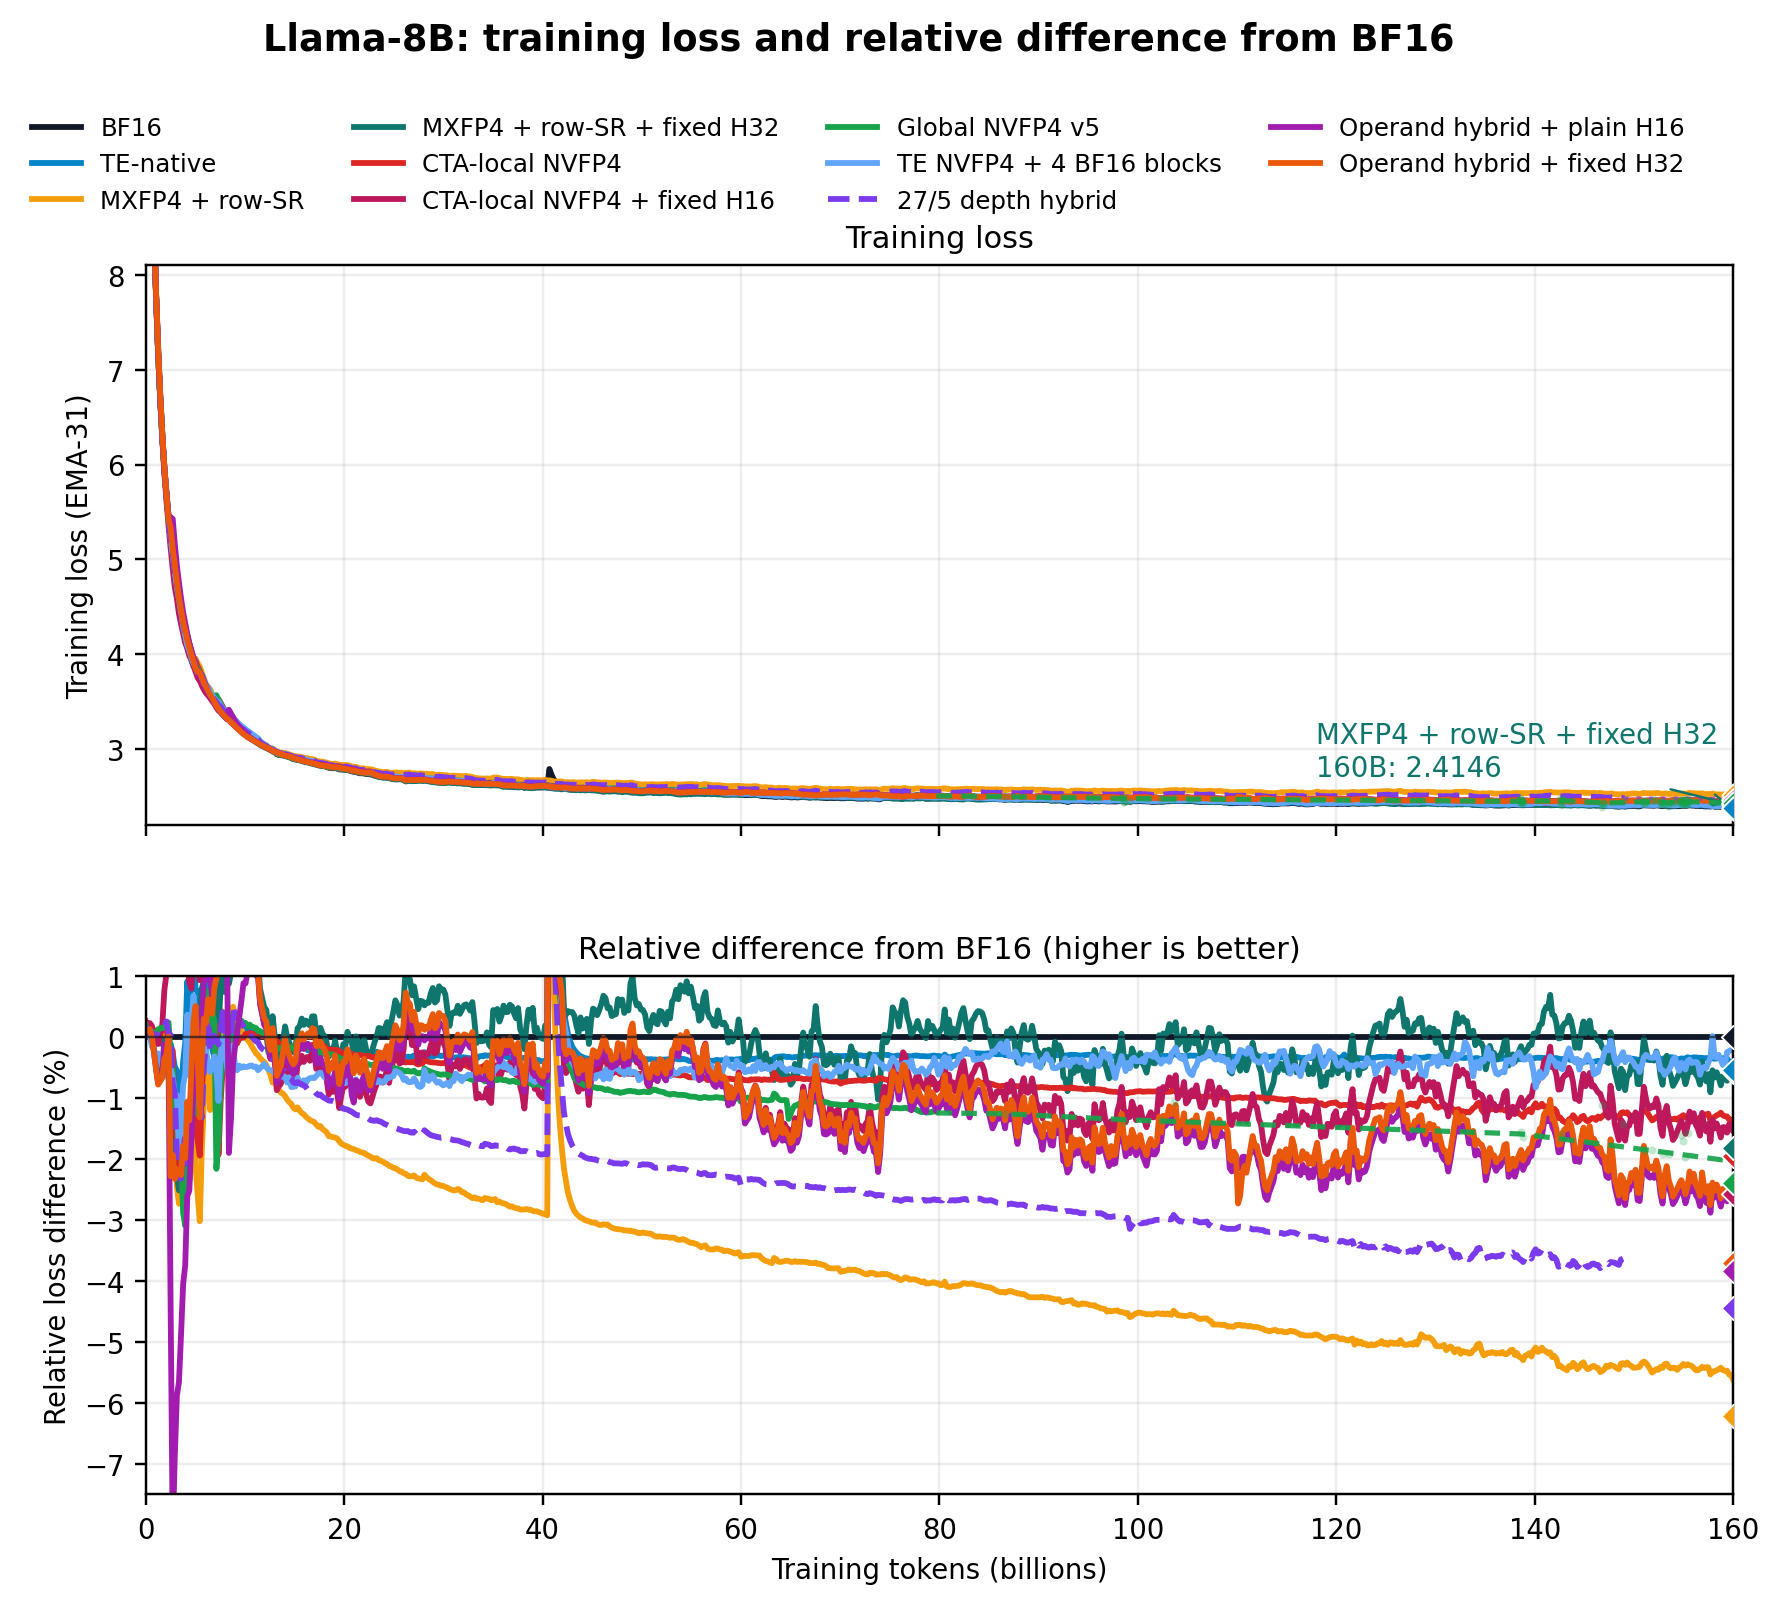
\includegraphics[width=0.98\textwidth]{figures/llama8b_160b_training_loss.png}
  \caption{Llama-8B training loss and relative difference from the BF16
  reference. Curves use EMA-31. Diamonds mark the final plotted endpoint.
  Sparse pure-v5 telemetry
  after step 19,000 is shown as exact anchors with a dashed robust locally
  weighted scatterplot smoothing (LOWESS) display fit. The fit is not used for
  endpoint values or comparisons. The dotted tail on the 27/5 depth hybrid
  marks a telemetry gap from its last continuous observations to the exact
  terminal point; it does not supply intermediate loss values.}
  \label{fig:llama8b-loss}
\end{figure}

Figure~\ref{fig:llama8b-loss-zoom} expands the final 40B-token window. It shows
the late loss separation at the same scale without extrapolating any route.

\begin{figure}[tbp]
  \centering
  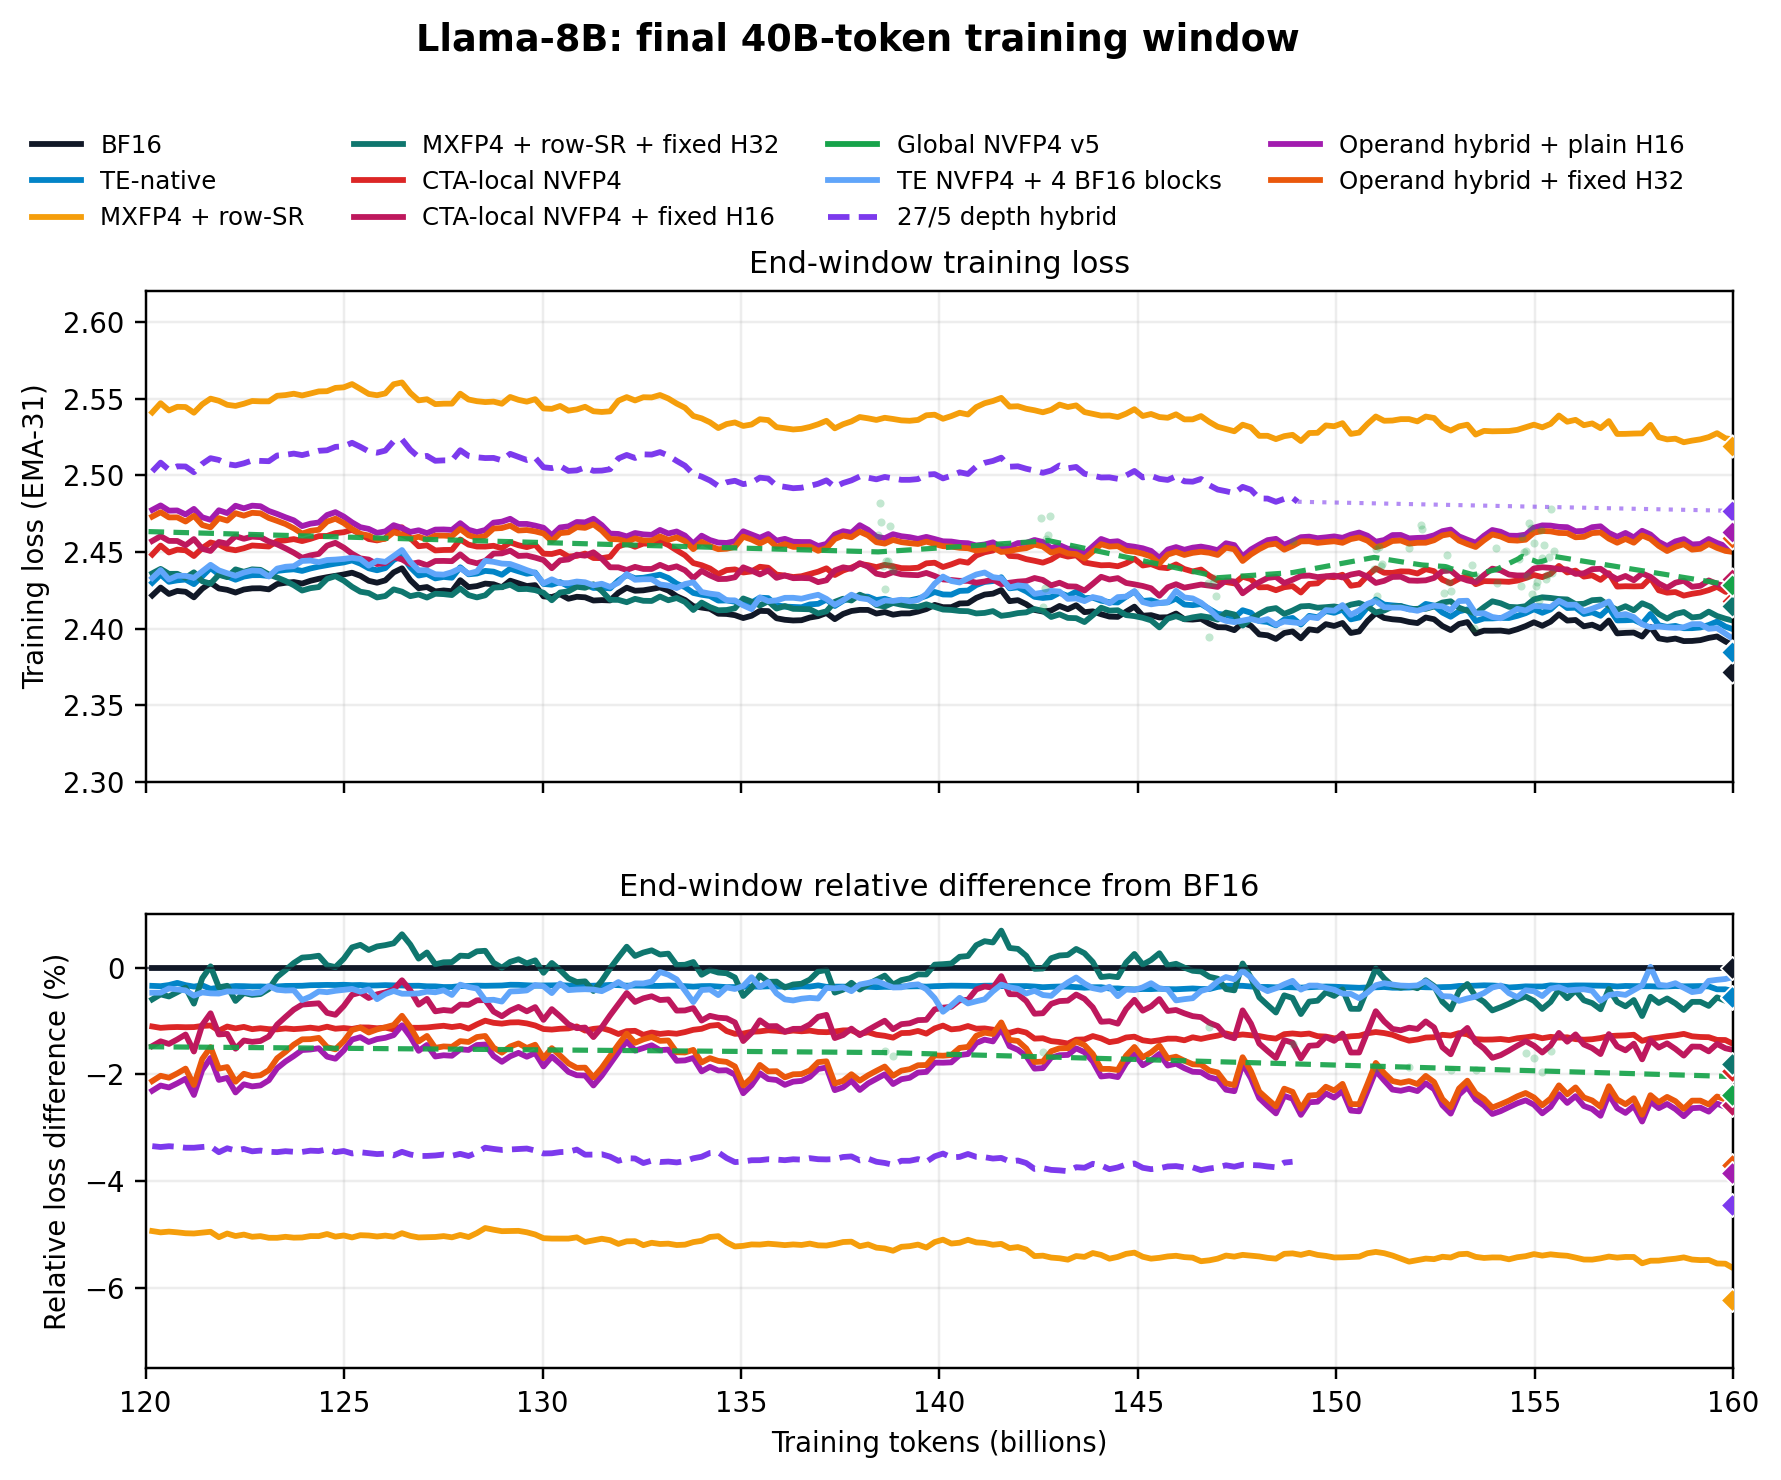
\includegraphics[width=0.98\textwidth]{figures/llama8b_160b_training_loss_zoom.png}
  \caption{Training loss from 120B to 160B tokens. Diamonds are exact logged
  endpoints. The dotted 27/5 tail marks an interval without intermediate
  telemetry and is not used in any comparison.}
  \label{fig:llama8b-loss-zoom}
\end{figure}

The TE route with four final BF16 blocks and the fixed-H32 operand hybrid each
contain 3,815 exact logged observations through step 38,140. Both trajectories
also have a sealed, resumable checkpoint at step 38,147.

\begin{table}[H]
  \centering
  \caption{Raw last logged minibatch loss at step 38,140 (159.97B tokens).
  ``Loss excess'' is relative to the unadjusted BF16 observation at that step.}
  \label{tab:training-endpoints}
  \begin{tabularx}{\textwidth}{Yrr}
    \toprule
    Route & Raw endpoint loss & Loss excess vs BF16 \\
    \midrule
    BF16 & 2.364637 & 0.00\% \\
    TE \nvfp{} + four final BF16 blocks & 2.385181 & 0.87\% \\
    TE-native \nvfp{} & 2.396353 & 1.34\% \\
    \mxfp{} + row-SR + fixed H32 & 2.414578 & 2.11\% \\
    \localcta{} & 2.417708 & 2.24\% \\
    Global \nvfp{} v5 & 2.428200 & 2.69\% \\
    \localcta{} + fixed H16 & 2.432642 & 2.88\% \\
    Operand hybrid + fixed H32 & 2.459305 & 4.00\% \\
    Operand hybrid + plain H16 & 2.462673 & 4.15\% \\
    27/5 depth hybrid & 2.476800 & 4.74\% \\
    \mxfp{} + row-SR & 2.519150 & 6.53\% \\
    \bottomrule
  \end{tabularx}
\end{table}

At step 38,140, the TE route with four final BF16 blocks is the closest
quantized trajectory to the raw BF16 observation, with 0.87\% excess, followed
by TE-native at 1.34\%. \mxfp{} with row-SR and fixed H32 is the closest custom
route at 2.11\%; it is 0.76\% above TE-native. The fixed-H32 operand hybrid
ends 1.85\% above the pure \mxfp{}-H32 route and 4.00\% above BF16.

Using tensors from the step-28,000 \mxfp{}+row-SR+fixed-H32 checkpoint, we replayed
Dgrad with \localcta{} and \mxfp{}. The surrounding replay configuration used
plain-H16 preconditioning only for Wgrad, which does not enter the scored
contraction. Against a BF16 replay, \localcta{} had lower Dgrad error energy
in all 288 layer--component comparisons; the geometric-mean
$E_{\mathrm{MX}}/E_{\mathrm{localCTA}}$ ratio was 1.292. The completed
plain-H16 operand hybrid nevertheless ends 1.99\% above \mxfp{}+row-SR+fixed H32 in
training loss. Appendix~\ref{app:dgrad-diagnostic} gives the capture and
aggregation contract.

\subsection{Validation loss}

Validation uses one fixed external stream with a complete document-and-token
provenance record. The converted and native evaluators agree exactly at the
full 8,192-token context. As a temporal control, BF16 validation NLL falls from
3.28327 at step 2,000 to 2.46052 at step 29,000. The paired difference is
$-0.82275$ NLL with a sequence-level standard error of 0.00371, placing the
comparison beyond the predeclared five-standard-error temporal gate. This
control establishes that the stream and evaluator recover the expected
learning order before comparing low-precision routes. Training loss is not
used as a substitute for validation loss.

Figure~\ref{fig:llama8b-validation} evaluates every available exact checkpoint
on that same stream. At the common step-38,000 cut, \mxfp{} with fixed H32 has
the lowest observed validation NLL, 2.422804. BF16 records 2.430206, the TE
route with four final BF16 blocks 2.437475, and TE-native 2.440488. The
fixed-H32 operand hybrid records 2.463842, compared with 2.460331 for
\localcta{} and 2.462074 for global \nvfp{} v5. Relative to BF16, the
\mxfp{}-H32, four-final-BF16-block, and operand-H32 differences are
$-0.305\%$, $+0.299\%$, and $+1.384\%$, respectively. These are observed
single-trajectory comparisons, not a one-factor isolation of H32 or
repeated-seed estimates.

\begin{figure}[tbp]
  \centering
  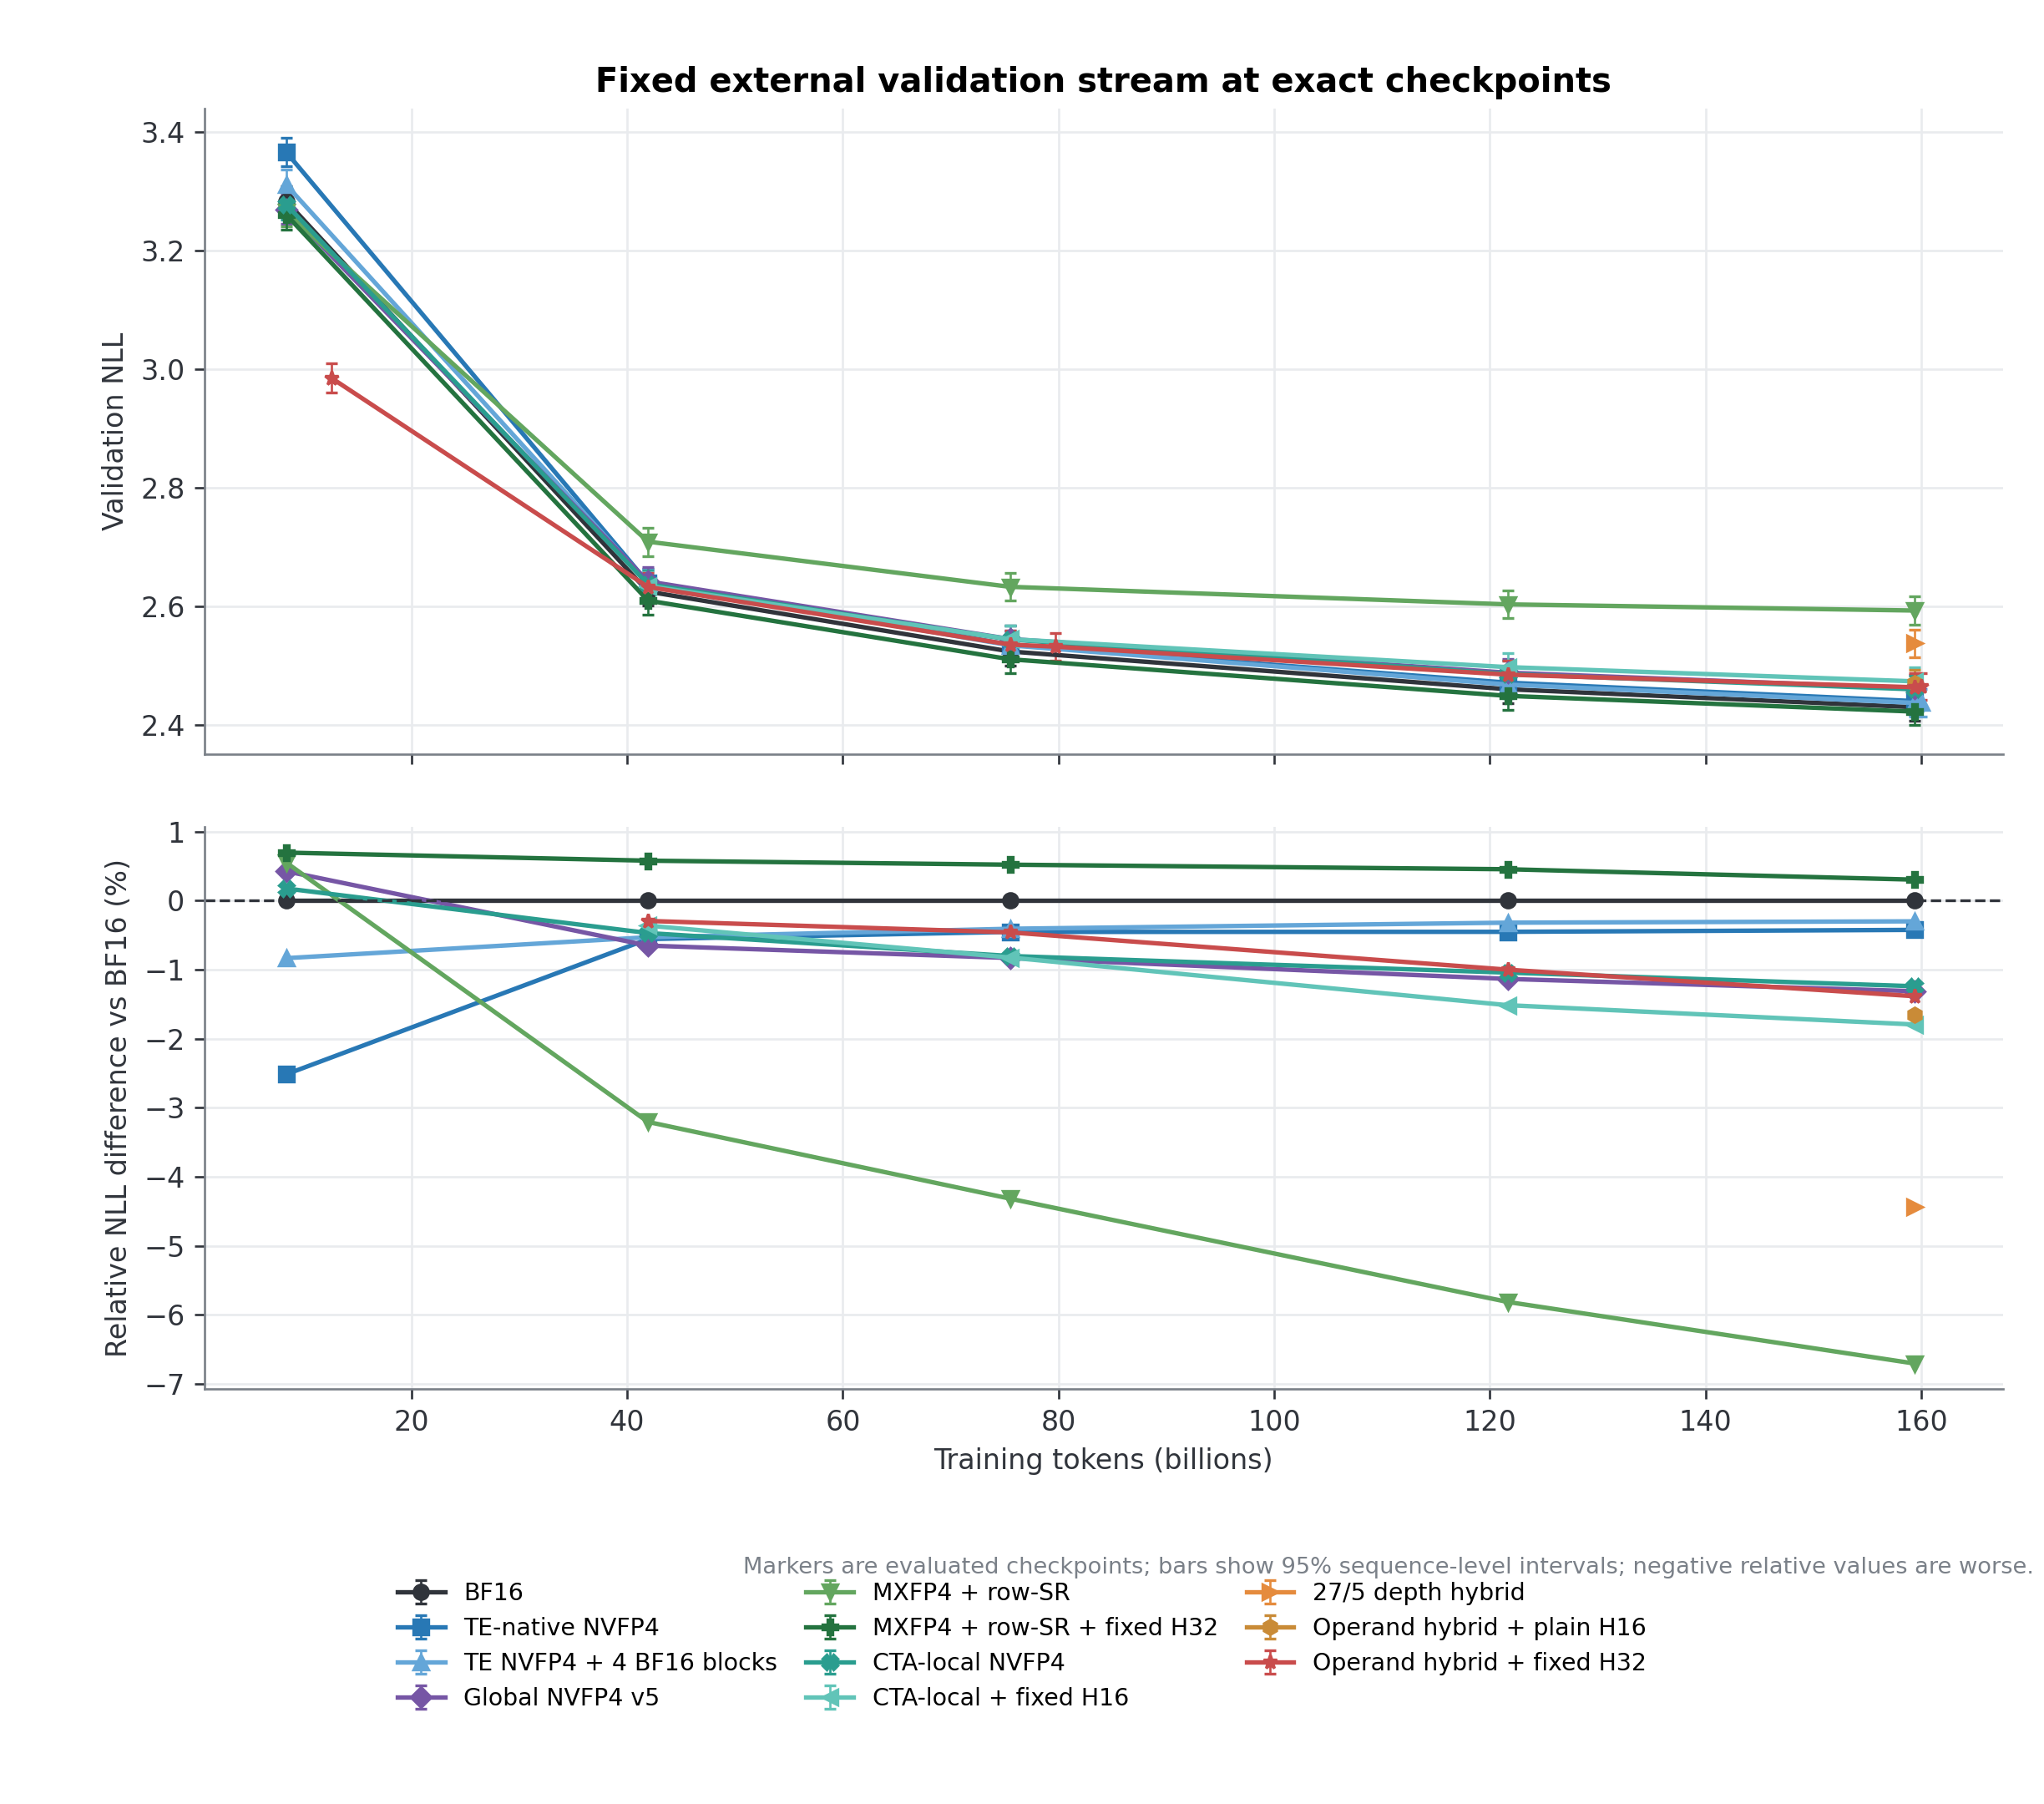
\includegraphics[width=0.98\textwidth]{figures/llama8b_validation_nll.png}
  \caption{Validation NLL on the fixed external stream at every available exact
  checkpoint. Error bars are 95\% sequence-level intervals. The lower panel
  reports $100(L_{\mathrm{BF16}}-L_{\mathrm{route}})/L_{\mathrm{BF16}}$ at
  exact shared steps, so negative values are worse than BF16. Lines connect
  measured checkpoints only; missing checkpoints are neither interpolated nor
  extrapolated.}
  \label{fig:llama8b-validation}
\end{figure}

\FloatBarrier

\subsection{How do the routes compare on downstream tasks?}

Each route is evaluated from its complete step-38,000 checkpoint using BF16
inference after verifying agreement with the training RoPE and RMSNorm
definitions. Eleven routes meet these criteria; routes without a complete
step-38,000 checkpoint are omitted. Every route uses the same MMLU,
HellaSwag, WinoGrande, and ARC-Challenge protocol.

\begin{table}[htbp]
  \centering
  \footnotesize
  \caption{Exact step-38,000 downstream scores (\%). MMLU and WinoGrande
  report accuracy; HellaSwag and ARC-Challenge report normalized accuracy.
  Shot counts are 5, 10, 5, and 25, respectively. Every route uses BF16
  inference after exact converted/native parity.}
  \label{tab:downstream-step38}
  \begin{adjustbox}{max width=\textwidth}
  \begin{tabular}{lrrrr}
    \toprule
    Route & MMLU & HellaSwag & WinoGrande & ARC-Challenge \\
    \midrule
    \input{data/llama8b_scaledrope_downstream_table_rows_20260903.tex}
  \end{tabular}
  \end{adjustbox}
\end{table}

The task ordering is not uniform. BF16 has the highest MMLU score, the
fixed-H32 operand hybrid has the highest WinoGrande score, and
\mxfp{}+row-SR+fixed H32 has the highest HellaSwag and ARC-Challenge scores.
Relative to that pure \mxfp{}-H32 route, the fixed-H32 operand hybrid differs
by $-1.66$, $-2.02$, $+0.79$, and $-2.39$ points on MMLU, HellaSwag,
WinoGrande, and ARC-Challenge, respectively. The four-final-BF16-block TE
route differs from BF16 by $-2.19$, $-0.53$, $-1.10$, and $+1.19$ points.
These are observations from one checkpoint per trajectory, not repeated-seed
estimates.

\begin{figure}[htbp]
  \centering
  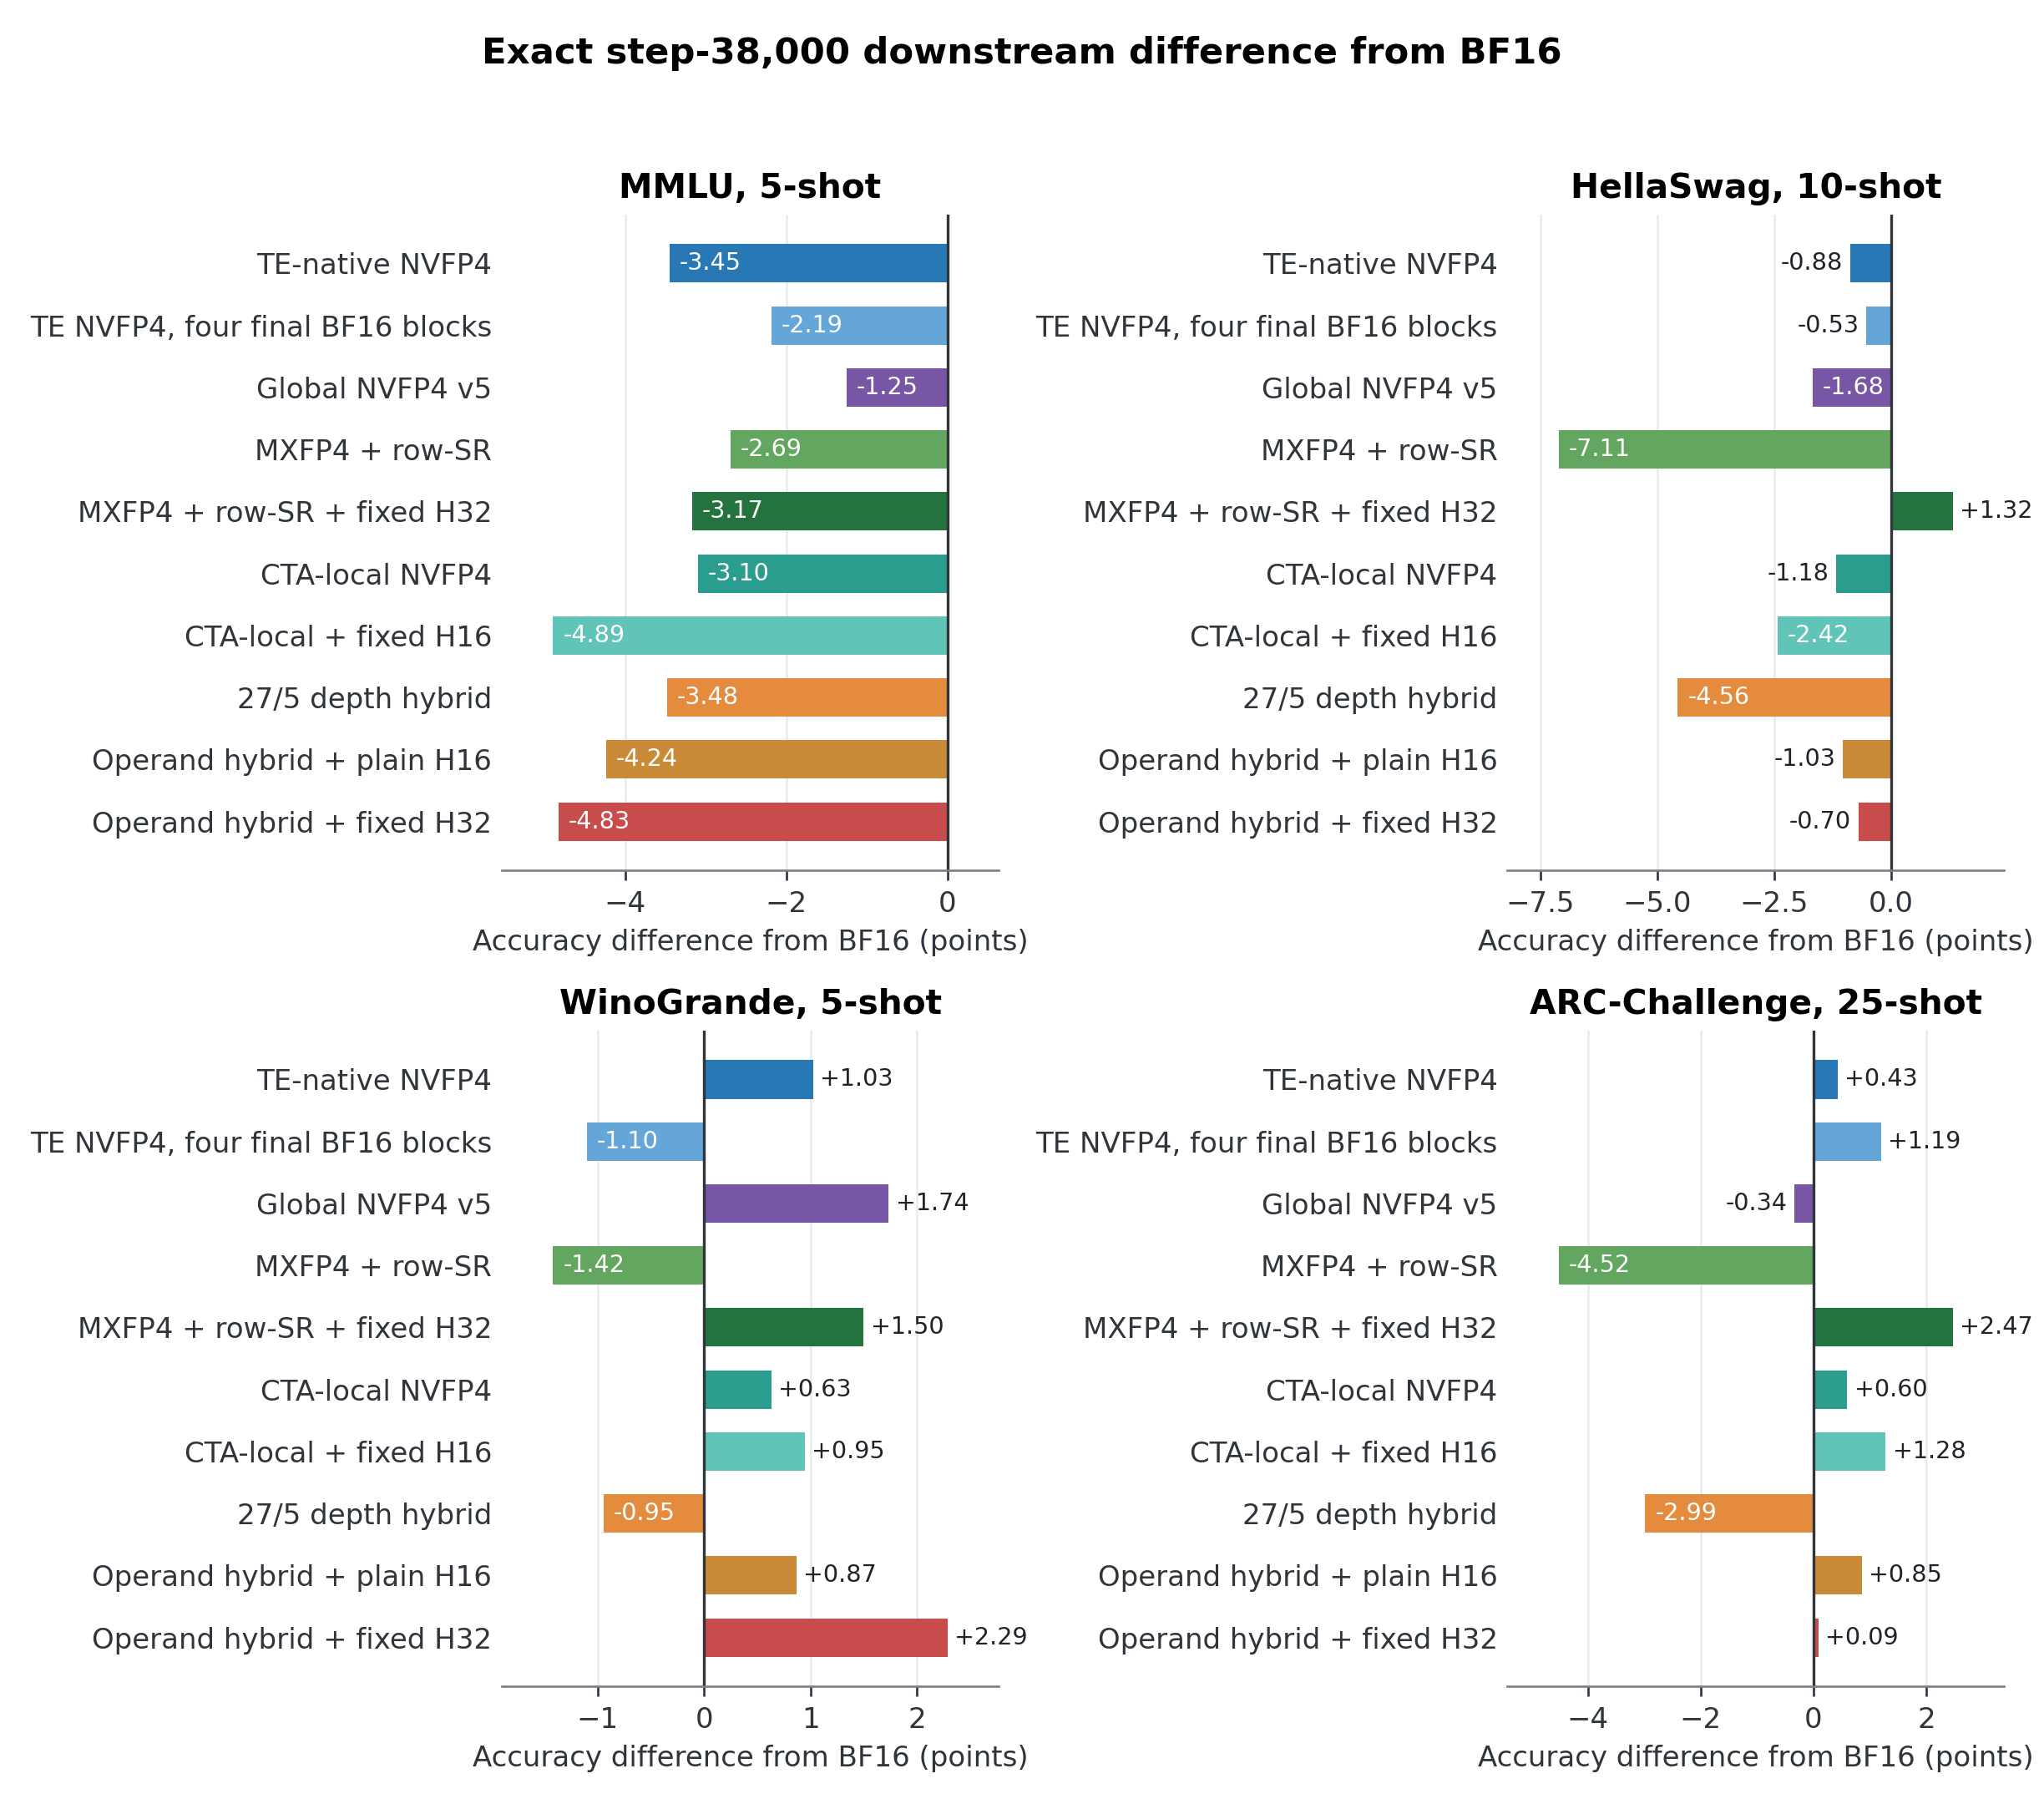
\includegraphics[width=0.98\textwidth]{figures/fp4_downstream_delta_bf16.png}
  \caption{Downstream reported-score difference from BF16 at exact step 38,000.
  Positive values exceed the BF16 score on that task. The absolute scores are
  reported in Table~\ref{tab:downstream-step38}.}
  \label{fig:downstream-delta}
\end{figure}
\FloatBarrier

\section{Discussion}

The measured TE routes track BF16 closely: TE-native and the
four-final-BF16-block route end 1.34\% and 0.87\% above the raw BF16 loss.
Their common probes reach 27.6K and 27.1K tokens/s/GPU. A separate
same-accelerator probe of the custom global \nvfp{} route reaches 32.5K
tokens/s/GPU; its long trajectory ends 2.69\% above BF16. TE-native \nvfp{}
and custom global \nvfp{} both use the tensor-global NVFP4 scale hierarchy;
the four-final-BF16-block route uses that hierarchy in its first 28 blocks.
The panel does not isolate the cost
of scaling from implementation and batch geometry, but it exposes the systems
constraint: a tensor-global maximum-absolute-value reduction creates a
completion dependency that the execution path must hide or pay.

Hadamard preconditioning is not uniformly beneficial across scale strategies.
The fixed-H32 \mxfp{} recipe retains 98.34\% of row-SR-only \mxfp{}
throughput while moving the raw endpoint excess from 6.53\% to 2.11\% and
validation NLL from 2.593146 to 2.422804. The fixed-H16 CTA-local recipe is
slower than CTA-local without the transform and has higher endpoint and
validation loss. These are comparisons between complete trajectories, not
experiments that isolate the effect of Hadamard preconditioning alone.

Neither tested hybrid dominates the strongest pure custom route. The
depth-wise hybrid and both operand-wise hybrids are slower and have higher
endpoint and validation loss than \mxfp{} with row-SR and fixed H32. A
controlled replay on identical saved tensors still finds lower Dgrad error for
CTA-local in all 288 tested layer--projection comparisons. The completed hybrid
trajectories do not preserve that operator-level advantage in endpoint or
validation loss.

\section{Conclusion}

Format-aware fusion makes the complete FP4 producer--consumer boundary the
unit of optimization. The TE routes give the closest observed training-loss
tracking, with measured tensor-global execution paths at 27.1--27.6K
tokens/s/GPU. Among the custom routes, \mxfp{} with row-gradient SR and
fixed-sign H32 Wgrad preconditioning gives the strongest measured
speed--quality point: 37.2K tokens/s/GPU, 86.3\% BF16 MFU, a 2.11\% raw
endpoint-loss excess, and the lowest observed validation NLL on the fixed
external data stream. Its
downstream ranking remains task dependent. Neither the tested depth-wise nor
operand-wise hybrid improves this combined point. The opposite outcomes of
Hadamard preconditioning under \mxfp{} and CTA-local scaling motivate choosing
the group of values sharing each scale, the rounding rule, and the
preconditioner jointly. UE5M3 results
on a separate model motivate a complementary next step: combine wider unsigned
block scales with local production or delayed global scaling
\cite{hu2026ue5m3}.


\section*{Code and Data Availability}

Code, pinned kernel sources, experiment recipes, and figure builders are
available at \url{https://github.com/MrHuff/mfu-fp4-training}. Project-authored
software is released under the MIT License. The original manuscript and
figures are released under CC BY 4.0; included third-party components retain
their own terms. Training corpora, tokenizer assets, model checkpoints, and
checkpoint metadata are not redistributed. The repository instead provides
hash-bound input schemas and the public recipes needed to bind authorized
local copies without recording credentials or private storage locations.

\section*{Generative-AI Disclosure}

OpenAI Codex provided substantial assistance with code development, experiment
orchestration, analysis, programmatic figure generation, and drafting and
editing this report. The system is not an author. The human author reviewed and
verified the code, experiments, numerical results, figures, citations, and
text and takes full responsibility for the content.

\bibliographystyle{plainnat}
\bibliography{references}

\appendix
\section{Implementation and Validation Notes}
\label{app:implementation}

The kernels specialize the production tensor shapes and define buffer
lifetimes across eager execution, recomputation, and CUDA Graph replay. QKV and
FFN producers emit both quantized orientations. Residual--RMSNorm preserves the
BF16 residual and exact row statistics required by backward. Each path is
checked against a higher-precision reference for outputs, input gradients,
weight gradients, relative RMS error, and zero fractions before model timing.

Row- and column-oriented scales are distinct numerical state, not
interchangeable layout metadata. Tensors returned to autograd cannot alias a
workspace whose lifetime ends with the producing stream. Delayed FP4 prefetch
has one owner and one release point. Distributed measurements use per-rank
timing and dispatch evidence because the slowest rank gates the step.

\subsection{Weight orientation and the fixed sign pattern}

The global-v5 path creates one 2D16 numerical weight
encoding and exposes it in both consumer layouts. The native 2D32 \mxfp{} path
follows the same orientation-consistency rule.

The signed-Hadamard paths use the fixed literal \texttt{0x00002817}. Under the
custom kernel's convention, a set bit denotes $+1$ and a clear bit denotes
$-1$. Bits 0--15 encode the same 16-entry sign vector that the pinned TE
implementation stores explicitly. The H32 implementation operates as two
16-value thread halves, and each half reuses this low-16-bit motif before the
cross-half shuffle. Thus H32 names the 32-value transform width, not a 32-bit
random mask: the reported H32 transform repeats one signed-H16 diagonal and
does not consume the literal's upper zero bits as positions 16--31. No signs
are drawn during training. The construction remains
orthogonal and preserves the unquantized Wgrad dot product because the
identical transform is paired on $X$ and $dY$. The experiments do not compare
this fixed vector with newly sampled signs and do not establish that the
particular diagonal is optimal.

Compilation and first-step kernel generation are excluded from steady-state
probe windows. Each measurement records device count, local batch, gradient
accumulation, seed, loss implementation, source revision, and metric window.
Each stochastic producer reserves one logical random-number interval, and the
ranked seed/subsequence state is checkpointed across resumes.

Table~\ref{tab:b300-snapshots} gives secondary production measurements. All
three use a BF16 output projection and compiled regular CE. Their batch
geometries and measurement windows differ, so they are not a one-factor
comparison.

\begin{table}[H]
  \centering
  \caption{Compiled-CE B300 production snapshots.
  BF16 MFU uses the B300's 2,250 TFLOP/s/GPU dense BF16 peak
  \cite{nvidia2026hgx}.}
  \label{tab:b300-snapshots}
  \begin{tabularx}{\textwidth}{Ylrrl}
    \toprule
    Route & LB/GA & Tokens/s/GPU & BF16 MFU & HBM/GPU \\
    \midrule
    \mxfp{} + row-SR & 4/4 & 39,306.59 & 101.17\% & 156.91--157.15 GiB \\
    \localcta{} & 8/2 & 36,728.43 & 94.54\% & 211.05--211.16 GiB \\
    27/5 depth hybrid & 8/2 & 37,394.00 & 96.25\% & 228.28--233.42 GiB \\
    \bottomrule
  \end{tabularx}
\end{table}

\section{Low-Precision Output Head: Negative Result}
\label{app:output-head}

This appendix records an engineering screen for which the exact low-precision
forward format was not preserved. The vocabulary projection has a large
forward GEMM and is therefore an attractive FP4 target. In the complete
trainer, however, the head also owns cross entropy, the hidden-state gradient,
the weight gradient, quantization, and saved-tensor lifetime. Accelerating one
GEMM did not accelerate that whole boundary.

MXFP8 below denotes an eight-bit microscaling format used for one
weight-gradient configuration.

\begin{table}[H]
  \centering
  \caption{Historical whole-trainer output-head screen. Deltas are paired
  within one experiment. The complete profiler metadata was not preserved, so
  rates are rounded and are not compared with the primary performance panel.}
  \label{tab:head-negative}
  \begin{tabularx}{\textwidth}{YrrY}
    \toprule
    Forward / hidden-state gradient / weight gradient & Tokens/s/GPU & Difference & Outcome \\
    \midrule
    BF16 / BF16 / BF16 & $\sim$34.00K & baseline & BF16 control \\
    lowp$^{\dagger}$ / BF16 / BF16 & $\sim$33.95K & $\sim-0.16\%$ & Loss differed from control \\
    lowp$^{\dagger}$ / BF16 / MXFP8 & $\sim$33.91K & $\sim-0.27\%$ & Loss and gradients differed \\
    \bottomrule
  \end{tabularx}
\end{table}

$^{\dagger}$ The experiment record preserves the backward choices and paired
rates but not the exact low-precision forward format. We therefore retain the
literal ``lowp'' label rather than assigning a more specific format after the
fact.

Both selective low-precision variants are slower than their matched BF16
control. The preserved record also says that neither reproduced the BF16
control loss, and that the MXFP8 weight-gradient configuration additionally
changed gradients; it
does not retain a publication-ready error magnitude, so we do not rank the
size of those numerical differences. These results support the selected
design: a BF16 output projection with compiled CE.

\section{Reproducibility}
\label{app:reproducibility}

\subsection{Report inputs}

The main training and performance tables and figures are generated from
checked-in data snapshots. The publication data directory contains the
training-loss series, same-accelerator performance aggregates, checkpoint
inventories, evaluation results, plotting programs, and a SHA-256 ledger.
Figure generators verify their declared inputs before writing an output. The
machine-readable recipe ledger records the route, precision policy, rounding
and preconditioning choices, batch geometry, seed when recovered, checkpoint
horizon, and evidence status for every experiment discussed in the paper.
Shared model, data, and optimizer fields are stored separately so that an
incomplete historical row cannot silently inherit a value from a newer run.

For display consistency, the historical BF16 and TE-native training-loss
curves in Figure~\ref{fig:llama8b-loss} use fixed offsets inferred from 41
matched steps in seed-42 controls. The raw series and adjustment remain in the
publication data.

The long-run curves combine only explicitly identified execution segments.
The \localcta{}+fixed-H16 and operand-hybrid trajectories each cross a
documented full-state resume boundary. Their manifests identify the source and
continuation ranges; no overlapping step is counted twice. Training-loss
observations for custom global NVFP4 are regular through step 19,000. The
configured Weights \& Biases run is no longer returned by the service, and the
dense local CSV named by the historical manifest was not present in any
recovered or released tree. Seventy-four exact observations survive after
step 19,000 in fragmented training logs. The largest missing sequence of
expected ten-step records runs from step 24,710 through step 33,000. The
dashed late line is a visual LOWESS fit through the surviving observations,
evaluated at the BF16 plotting steps. It is never used to compute a reported numeric
endpoint, table entry, or statistic.

\subsection{Checkpoint and evaluator contract}

Training comparisons use exact shared steps. Custom-route values are raw
observations. Downstream comparisons use literal step-38,000
checkpoints; a terminal, nearby, or checkpoint from a different training run
is never substituted. Distributed checkpoints must contain all expected
shards and pass conversion checks before evaluation.

The evaluator must reproduce the training model's RoPE and RMSNorm semantics.
The Llama-3.1 8B training configuration uses base $500{,}000$ and the
long-context RoPE scaling parameters $(8,1,4,8192)$. An earlier evaluator
disabled this scaling in both the converted-checkpoint evaluator and native
TorchTitan reference. Agreement between those two implementations therefore
did not establish agreement with the training model. Results from that
evaluator are excluded.

An earlier validation stream used the correct model semantics but failed a
data-source robustness check: apparent route ordering changed when examples
came from different contiguous regions of the source datasets. Those values
are also excluded. The replacement stream was constructed afresh from
deterministic windows in the 90--95\% physical sample range of the DCLM and
OLMo-without-DCLM components. Documents are deduplicated by raw-text SHA-256,
combined at an 82/18 token ratio, globally hash-shuffled, and only then packed
and sharded. Thus no GPU worker is restricted to one source or contiguous
region of source data.

The replacement fixed validation stream contains 768 sequences of 8,193 tokens, yielding
6,291,456 scored next-token targets. It is tokenized once with the pinned
Llama-3.1 tokenizer and reused byte-for-byte for every checkpoint. We call it
a \emph{fixed external validation stream}, not a held-out split, because zero
document overlap across every historical training trajectory has not been
proven. Its source ledger contains 4,597 documents with
4,597 unique raw-text hashes. Before reporting route comparisons, the
corrected checkpoint evaluator must agree exactly with the native TorchTitan
model at the full 8,192-token context, and a late BF16 checkpoint must improve
over an early BF16 checkpoint by more than five sequence-level standard
errors. Both checks pass. The converted checkpoint and native TorchTitan model
agree exactly at full context for the step-2,000 and step-29,000 BF16
checkpoints. Their validation NLL values are 3.283272 and 2.460520,
respectively; the paired late-minus-early difference is $-0.822753$ with
sequence-level standard error 0.003708.

Downstream evaluation uses BF16 inference and one evaluator configuration for
all routes. MMLU is 5-shot, HellaSwag 10-shot, WinoGrande 5-shot, and
ARC-Challenge 25-shot; HellaSwag and ARC report normalized accuracy. A route
enters the common panel only after the exact checkpoint and corrected model
semantics are verified.

\subsection{Historical execution identity}

Historical experiments are bound to the code, submodule, kernel asset,
checkpoint, and output identities recovered for that execution. The current
source and runtime tips are not assigned retroactively to an older run. Where
a field was not recovered, the ledger records it as unknown rather than
guessing the nearest commit. Complete identifiers and content digests are in
the publication data ledger rather than the narrative.

The custom global NVFP4 path uses one orientation-consistent 2D16 weight
encoding. The code used by the completed \mxfp{}+row-SR+fixed-H32 run is
content-verified in its run manifest. The \localcta{}+fixed-H16 and
operand-wise plain-H16 trajectories each join verified execution segments at
an exact full-state checkpoint. Their manifests record implementation changes,
segment boundaries, and checkpoint state.

\subsection{Controlled Dgrad diagnostic}
\label{app:dgrad-diagnostic}

The operand-format diagnostic uses tensors from the step-28,000 checkpoint of
the completed \mxfp{}+row-SR+fixed-H32 trajectory. It computes Dgrad with
\mxfp{} and \localcta{} against the corresponding BF16 result. The diagnostic
configures a paired plain-H16 transform for Wgrad only; that transform does
not enter the scored Dgrad contraction and is not part of the comparison.

For each captured tensor, four stochastic candidate tensors are averaged
before computing
\begin{equation}
  E=\sum_i\left(\widehat{dX}_i-dX_i^{\mathrm{BF16}}\right)^2.
\end{equation}
The capture covers three
sequence-2,048 batches, QKV, attention-output, and FFN projections in all 32
blocks, and an independently seeded stochastic-rounding generator rather than
the training run's saved generator state. This gives 96 layer--component
comparisons per batch and 288 in total.
\localcta{} has lower error energy in all 288 comparisons. Giving each tensor
equal weight, the cross-capture geometric mean of
$E_{\mathrm{MX}}/E_{\mathrm{localCTA}}$ is 1.292.

\subsection{Excluded experiments}

The custom global \nvfp{}/\mxfp{} depth hybrid remains outside the common endpoint panels because
it diverged and retained only 16 of 32 terminal shards. The TE route with four
final BF16 blocks and the fixed-H32 operand hybrid both completed 160B-token
trajectories with resumable final checkpoints and are included in the endpoint
panels.

Diagnostic screens are also excluded from the common panels. The
low-precision output-head configurations produced no stable model-level
speedup. A \localcta{} transform screen resumed near the end of training under
a changed runtime, so it is not a causal comparison. The superseded downstream
evaluator omitted training-time RoPE scaling, while the superseded validation
stream was sensitive to the contiguous source-data region selected. Their
records are retained for audit, not used as scientific endpoints.

Run \texttt{make} in the report directory to regenerate the figures and PDF.
The checked-in data README lists each source file, generator, and verification
command; \texttt{data/SHA256SUMS} binds the publication inputs.

\subsection{Code and data availability}
\label{app:code-release}

Code, pinned kernel sources, experiment recipes, evaluation tools, and figure
builders are available at
\url{https://github.com/MrHuff/mfu-fp4-training}. Project-authored software is
released under the MIT License. The original manuscript and figures are
released under CC BY 4.0; included third-party components retain their own
terms. Training corpora, tokenizer assets, model checkpoints, and checkpoint
metadata are not redistributed. The repository instead provides hash-bound
input schemas and public recipes for binding authorized local copies without
recording credentials or private storage locations.


\end{document}
